\begin{frame}[fragile]{In-memory representation stage}
\begin{itemize}
\setlength{\itemindent}{-1.0em}
    \item We use a \cred{Boost Graph} Library:  \cblue{generic programming},  \cblue{open-source} and \cblue{header-only} library {
\begin{minted}[linenos=false, frame=single, framesep=2mm,fontsize=\scriptsize]{cpp}
adjacency_list<OutEdgeList, VertexList, Directed, 
               VertexProperties, EdgeProperties, GraphProperties, EdgeList>
\end{minted}      
    }
\item We use an \cred{undirected graph} with values in \cpipes{pipes}/\cnodes{nodes} assigned via the graph properties

% FORKAROL: read for the generic explanation and to open the talk about the given caractheristics of the pipes and nodes by suing boost::graph
% https://www.boost.org/doc/libs/1_82_0/libs/graph/doc/index.html

\begin{center}

\begin{minipage}{0.51\textwidth}
\vspace{-0.25cm}
\begin{minted}[linenos=true,numbersep=1pt,frame=lines,framesep=0.5mm,fontsize=\notsotiny, bgcolor=background]{cpp}
 using namespace boost;
 using graph_type = adjacency_list< listS, vecS,  
                                    undirectedS,
            vertex_properties, edge_properties>;
           
 graph_type graph;
\end{minted}  
\vspace{-0.75cm}
\begin{minted}[linenos=true,numbersep=1pt,frame=lines,framesep=0.5mm,fontsize=\notsotiny]{cpp}
 enum class edge_type {
     pipe,
     resistor,
     compressor,
     regulator,
     valve,
};
 \end{minted}
\vfill
\end{minipage}%
\hfill
\begin{minipage}{0.38\textwidth}
    \begin{minted}[linenos=true,numbersep=1pt,frame=lines,framesep=1.1 mm,fontsize=\notsotiny, bgcolor=background]{cpp}
 struct vertex_properties {
     std::string     name;
     int             number;
     double          height;
     vector_t        gas_mixture;   
 };

 struct edge_properties {
     edge_type   type;
     int         number;
     double      length;
     double      diameter;
     double      friction_factor;
 };  
\end{minted}    
\end{minipage}%    
\end{center}

\item Matrices directly built from graph: Incidence matrix, Resistance matrix, Inertia term
\end{itemize}
\end{frame}

%----------------------------------------------------------------
\begin{frame}[fragile]{Graph initialization}
\begin{itemize}
    \item Graph representation and \cnodes{nodes} specification

    \begin{center}       
    \begin{minipage}{0.25\textwidth}
            \begin{center}
            % Graphic for TeX using PGF
% Title: /home/karol/Documents/UNIVERSITA/POLITO/PRESENTATIONS/SHIMMER_2024_01/img_code/pipe_network.dia
% Creator: Dia v0.97.3
% CreationDate: Mon Jan 22 14:43:56 2024
% For: karol
% \usepackage{tikz}
% The following commands are not supported in PSTricks at present
% We define them conditionally, so when they are implemented,
% this pgf file will use them.
\ifx\du\undefined
  \newlength{\du}
\fi
\setlength{\du}{11\unitlength}
\begin{tikzpicture}[even odd rule]
\pgftransformxscale{1.000000}
\pgftransformyscale{-1.000000}
\definecolor{dialinecolor}{rgb}{0.000000, 0.000000, 0.000000}
\pgfsetstrokecolor{dnode}
\pgfsetstrokeopacity{1.000000}
\definecolor{diafillcolor}{rgb}{1.000000, 1.000000, 1.000000}
\pgfsetfillcolor{diafillcolor}
\pgfsetfillopacity{1.000000}
\pgfsetlinewidth{0.100000\du}
\pgfsetdash{}{0pt}
\pgfsetmiterjoin
\definecolor{diafillcolor}{rgb}{1.000000, 1.000000, 1.000000}
\pgfsetfillcolor{diafillcolor}
\pgfsetfillopacity{1.000000}
\pgfpathellipse{\pgfpoint{8.693572\du}{5.676288\du}}{\pgfpoint{0.693572\du}{0\du}}{\pgfpoint{0\du}{0.676288\du}}
\pgfusepath{fill}
\definecolor{dialinecolor}{rgb}{0.937255, 0.000000, 0.701961}
\pgfsetstrokecolor{dnode}
\pgfsetstrokeopacity{1.000000}
\pgfpathellipse{\pgfpoint{8.693572\du}{5.676288\du}}{\pgfpoint{0.693572\du}{0\du}}{\pgfpoint{0\du}{0.676288\du}}
\pgfusepath{stroke}
% setfont left to latex
% setfont left to latex
\definecolor{dialinecolor}{rgb}{0.000000, 0.000000, 0.000000}
\pgfsetstrokecolor{dnode}
\pgfsetstrokeopacity{1.000000}
\definecolor{diafillcolor}{rgb}{0.000000, 0.000000, 0.000000}
\pgfsetfillcolor{diafillcolor}
\pgfsetfillopacity{1.000000}
\node[anchor=base,inner sep=0pt, outer sep=0pt,color=dnode] at (8.693572\du,5.961288\du){0};
\pgfsetlinewidth{0.100000\du}
\pgfsetdash{}{0pt}
\pgfsetmiterjoin
\definecolor{diafillcolor}{rgb}{1.000000, 1.000000, 1.000000}
\pgfsetfillcolor{diafillcolor}
\pgfsetfillopacity{1.000000}
\pgfpathellipse{\pgfpoint{8.693572\du}{9.676288\du}}{\pgfpoint{0.693572\du}{0\du}}{\pgfpoint{0\du}{0.676288\du}}
\pgfusepath{fill}
\definecolor{dialinecolor}{rgb}{0.937255, 0.000000, 0.701961}
\pgfsetstrokecolor{dnode}
\pgfsetstrokeopacity{1.000000}
\pgfpathellipse{\pgfpoint{8.693572\du}{9.676288\du}}{\pgfpoint{0.693572\du}{0\du}}{\pgfpoint{0\du}{0.676288\du}}
\pgfusepath{stroke}
% setfont left to latex
% setfont left to latex
\definecolor{dialinecolor}{rgb}{0.000000, 0.000000, 0.000000}
\pgfsetstrokecolor{dialinecolor}
\pgfsetstrokeopacity{1.000000}
\definecolor{diafillcolor}{rgb}{0.000000, 0.000000, 0.000000}
\pgfsetfillcolor{diafillcolor}
\pgfsetfillopacity{1.000000}
\node[anchor=base,inner sep=0pt, outer sep=0pt,color=dnode] at (8.693572\du,9.961288\du){1};
\pgfsetlinewidth{0.100000\du}
\pgfsetdash{}{0pt}
\pgfsetmiterjoin
\definecolor{diafillcolor}{rgb}{1.000000, 1.000000, 1.000000}
\pgfsetfillcolor{diafillcolor}
\pgfsetfillopacity{1.000000}
\pgfpathellipse{\pgfpoint{6.753572\du}{13.676288\du}}{\pgfpoint{0.753572\du}{0\du}}{\pgfpoint{0\du}{0.676288\du}}
\pgfusepath{fill}
\definecolor{dialinecolor}{rgb}{0.937255, 0.000000, 0.701961}
\pgfsetstrokecolor{dnode}
\pgfsetstrokeopacity{1.000000}
\pgfpathellipse{\pgfpoint{6.753572\du}{13.676288\du}}{\pgfpoint{0.753572\du}{0\du}}{\pgfpoint{0\du}{0.676288\du}}
\pgfusepath{stroke}
% setfont left to latex
% setfont left to latex
\definecolor{dialinecolor}{rgb}{0.000000, 0.000000, 0.000000}
\pgfsetstrokecolor{dialinecolor}
\pgfsetstrokeopacity{1.000000}
\definecolor{diafillcolor}{rgb}{0.000000, 0.000000, 0.000000}
\pgfsetfillcolor{diafillcolor}
\pgfsetfillopacity{1.000000}
\node[anchor=base,inner sep=0pt, outer sep=0pt,color=dnode] at (6.753572\du,13.961288\du){2};
\pgfsetlinewidth{0.100000\du}
\pgfsetdash{}{0pt}
\pgfsetmiterjoin
\definecolor{diafillcolor}{rgb}{1.000000, 1.000000, 1.000000}
\pgfsetfillcolor{diafillcolor}
\pgfsetfillopacity{1.000000}
\pgfpathellipse{\pgfpoint{14.693572\du}{13.676288\du}}{\pgfpoint{0.693572\du}{0\du}}{\pgfpoint{0\du}{0.676288\du}}
\pgfusepath{fill}
\definecolor{dialinecolor}{rgb}{0.937255, 0.000000, 0.701961}
\pgfsetstrokecolor{dnode}
\pgfsetstrokeopacity{1.000000}
\pgfpathellipse{\pgfpoint{14.693572\du}{13.676288\du}}{\pgfpoint{0.693572\du}{0\du}}{\pgfpoint{0\du}{0.676288\du}}
\pgfusepath{stroke}
% setfont left to latex
% setfont left to latex
\definecolor{dialinecolor}{rgb}{0.000000, 0.000000, 0.000000}
\pgfsetstrokecolor{dialinecolor}
\pgfsetstrokeopacity{1.000000}
\definecolor{diafillcolor}{rgb}{0.000000, 0.000000, 0.000000}
\pgfsetfillcolor{diafillcolor}
\pgfsetfillopacity{1.000000}
\node[anchor=base,inner sep=0pt, outer sep=0pt,color=dnode] at (14.693572\du,13.961288\du){4};
\pgfsetlinewidth{0.100000\du}
\pgfsetdash{}{0pt}
\pgfsetmiterjoin
\definecolor{diafillcolor}{rgb}{1.000000, 1.000000, 1.000000}
\pgfsetfillcolor{diafillcolor}
\pgfsetfillopacity{1.000000}
\pgfpathellipse{\pgfpoint{10.693572\du}{13.676288\du}}{\pgfpoint{0.693572\du}{0\du}}{\pgfpoint{0\du}{0.676288\du}}
\pgfusepath{fill}
\definecolor{dialinecolor}{rgb}{0.937255, 0.000000, 0.701961}
\pgfsetstrokecolor{dnode}
\pgfsetstrokeopacity{1.000000}
\pgfpathellipse{\pgfpoint{10.693572\du}{13.676288\du}}{\pgfpoint{0.693572\du}{0\du}}{\pgfpoint{0\du}{0.676288\du}}
\pgfusepath{stroke}
% setfont left to latex
% setfont left to latex
\definecolor{dialinecolor}{rgb}{0.000000, 0.000000, 0.000000}
\pgfsetstrokecolor{dialinecolor}
\pgfsetstrokeopacity{1.000000}
\definecolor{diafillcolor}{rgb}{0.000000, 0.000000, 0.000000}
\pgfsetfillcolor{diafillcolor}
\pgfsetfillopacity{1.000000}
\node[anchor=base,inner sep=0pt, outer sep=0pt,color=dnode] at (10.693572\du,13.961288\du){3};
\pgfsetlinewidth{0.050000\du}
\pgfsetdash{}{0pt}
\pgfsetbuttcap
{
\definecolor{diafillcolor}{rgb}{0.000000, 0.501961, 0.501961}
\pgfsetfillcolor{diafillcolor}
\pgfsetfillopacity{1.000000}
% was here!!!
\definecolor{dialinecolor}{rgb}{0.000000, 0.501961, 0.501961}
\pgfsetstrokecolor{dpipe}
\pgfsetstrokeopacity{1.000000}
\draw (8.693572\du,6.351417\du)--(8.693570\du,9.000000\du);
}
\pgfsetlinewidth{0.050000\du}
\pgfsetdash{}{0pt}
\pgfsetbuttcap
{
\definecolor{diafillcolor}{rgb}{0.000000, 0.501961, 0.501961}
\pgfsetfillcolor{diafillcolor}
\pgfsetfillopacity{1.000000}
% was here!!!
\definecolor{dialinecolor}{rgb}{0.000000, 0.501961, 0.501961}
\pgfsetstrokecolor{dpipe}
\pgfsetstrokeopacity{1.000000}
\draw (8.693570\du,10.352600\du)--(6.753570\du,13.000000\du);
}
\pgfsetlinewidth{0.050000\du}
\pgfsetdash{}{0pt}
\pgfsetbuttcap
{
\definecolor{diafillcolor}{rgb}{0.000000, 0.501961, 0.501961}
\pgfsetfillcolor{diafillcolor}
\pgfsetfillopacity{1.000000}
% was here!!!
\definecolor{dialinecolor}{rgb}{0.000000, 0.501961, 0.501961}
\pgfsetstrokecolor{dpipe}
\pgfsetstrokeopacity{1.000000}
\draw (8.693570\du,10.352600\du)--(10.693600\du,13.000000\du);
}
\pgfsetlinewidth{0.050000\du}
\pgfsetdash{}{0pt}
\pgfsetbuttcap
{
\definecolor{diafillcolor}{rgb}{0.000000, 0.501961, 0.501961}
\pgfsetfillcolor{diafillcolor}
\pgfsetfillopacity{1.000000}
% was here!!!
\definecolor{dialinecolor}{rgb}{0.000000, 0.501961, 0.501961}
\pgfsetstrokecolor{dpipe}
\pgfsetstrokeopacity{1.000000}
\draw (10.000000\du,13.676300\du)--(7.507140\du,13.676300\du);
}
\pgfsetlinewidth{0.050000\du}
\pgfsetdash{}{0pt}
\pgfsetbuttcap
{
\definecolor{diafillcolor}{rgb}{0.000000, 0.501961, 0.501961}
\pgfsetfillcolor{diafillcolor}
\pgfsetfillopacity{1.000000}
% was here!!!
\definecolor{dialinecolor}{rgb}{0.000000, 0.501961, 0.501961}
\pgfsetstrokecolor{dpipe}
\pgfsetstrokeopacity{1.000000}
\draw (11.387100\du,13.676300\du)--(14.000000\du,13.676300\du);
}
% setfont left to latex
% setfont left to latex
\definecolor{dialinecolor}{rgb}{0.000000, 0.501961, 0.501961}
\pgfsetstrokecolor{dialinecolor}
\pgfsetstrokeopacity{1.000000}
\definecolor{diafillcolor}{rgb}{0.000000, 0.501961, 0.501961}
\pgfsetfillcolor{diafillcolor}
\pgfsetfillopacity{1.000000}
\node[anchor=base west,inner sep=0pt,outer sep=0pt,color=dpipe] at (7.5000000\du,8.000000\du){0};
% setfont left to latex
% setfont left to latex
\definecolor{dialinecolor}{rgb}{0.000000, 0.501961, 0.501961}
\pgfsetstrokecolor{dialinecolor}
\pgfsetstrokeopacity{1.000000}
\definecolor{diafillcolor}{rgb}{0.000000, 0.501961, 0.501961}
\pgfsetfillcolor{diafillcolor}
\pgfsetfillopacity{1.000000}
\node[anchor=base west,inner sep=0pt,outer sep=0pt,color=dpipe] at (6.5000000\du,12.000000\du){3};
% setfont left to latex
% setfont left to latex
\definecolor{dialinecolor}{rgb}{0.000000, 0.501961, 0.501961}
\pgfsetstrokecolor{dialinecolor}
\pgfsetstrokeopacity{1.000000}
\definecolor{diafillcolor}{rgb}{0.000000, 0.501961, 0.501961}
\pgfsetfillcolor{diafillcolor}
\pgfsetfillopacity{1.000000}
\node[anchor=base west,inner sep=0pt,outer sep=0pt,color=dpipe] at (10.5000000\du,12.000000\du){1};
% setfont left to latex
% setfont left to latex
\definecolor{dialinecolor}{rgb}{0.000000, 0.501961, 0.501961}
\pgfsetstrokecolor{dialinecolor}
\pgfsetstrokeopacity{1.000000}
\definecolor{diafillcolor}{rgb}{0.000000, 0.501961, 0.501961}
\pgfsetfillcolor{diafillcolor}
\pgfsetfillopacity{1.000000}
\node[anchor=base west,inner sep=0pt,outer sep=0pt,color=dpipe] at (8.450000\du,14.900000\du){2};
% setfont left to latex
% setfont left to latex
\definecolor{dialinecolor}{rgb}{0.000000, 0.501961, 0.501961}
\pgfsetstrokecolor{dialinecolor}
\pgfsetstrokeopacity{1.000000}
\definecolor{diafillcolor}{rgb}{0.000000, 0.501961, 0.501961}
\pgfsetfillcolor{diafillcolor}
\pgfsetfillopacity{1.000000}
\node[anchor=base west,inner sep=0pt,outer sep=0pt,color=dpipe] at (12.590000\du,14.895000\du){4};
\end{tikzpicture}
    
            \end{center}
    \end{minipage}
    \hfill
    \begin{minipage}{0.65\textwidth}
        \begin{table}
        \footnotesize
        \begin{tabular}{ccrrrcccc}
        &&&&&&&&\\
        \hline 
        &  & \multicolumn{3}{c}{Node properties}  & & \multicolumn{3}{c}{Mixture composition} \\ \cline{3-5} \cline{7-9}     
        \multirow{5}{*}{\rotatebox[origin=c]{90}{\cnodes{Nodes}}} 
        &           & G[kg/s] &p[Pa] &H[m]  && CH4 & N2& \dots \\ \hline
        &\cnodes{0} &	5000  & -60  &10.0  && -& -& -\\
        &\cnodes{1} &	0	  &  20  &20.0  && -& - & -\\
        &\cnodes{2} &	0	  &  25  &30.0  && -& - & -\\ 
        &\cnodes{3} &	0	  &  35  &40.0  && -& - & -\\ 
        &\cnodes{4} &	0	  &  50  &50.0  && -& - & -\\
        \hline
        &&&&&&&&\\
        \end{tabular}
        \end{table}
    \end{minipage}
   \end{center}
\item Insertion of vertices using the $boost::add\_vertex$ function
    \begin{center}
    \begin{minted}[linenos=true,numbersep=1pt,frame=lines,framesep=2mm,fontsize=\scriptsize, bgcolor=background]{cpp}
    // Insert station config (name, no., pressure, flux, height)
    auto v0 = add_vertex( { "Station 0", 0, 5e3,-60, 10}, graph) );
    auto v1 = add_vertex( { "Station 1", 1,  0,  20, 20}, graph) );
    auto v2 = add_vertex( { "Station 2", 2,  0,  25, 30}, graph) );
    auto v3 = add_vertex( { "Station 3", 3,  0,  35, 40}, graph) );
    auto v4 = add_vertex( { "Station 4", 4,  0,  50, 50}, graph) );

    std::vector<vertex_descriptor> vds = {v0,v1,v2,v3,v4};  
    \end{minted}
        
    \end{center}

\end{itemize}

\end{frame}
%----------------------------------------------------------------
\begin{frame}[fragile]{Graph initialization}
\begin{itemize}
    \item Graph representation and \cpipes{pipes} specification   
        \begin{center}
        \begin{minipage}{0.25\textwidth}
            \begin{center}
            % Graphic for TeX using PGF
% Title: /home/karol/Documents/UNIVERSITA/POLITO/PRESENTATIONS/SHIMMER_2024_01/img_code/pipe_network.dia
% Creator: Dia v0.97.3
% CreationDate: Mon Jan 22 14:43:56 2024
% For: karol
% \usepackage{tikz}
% The following commands are not supported in PSTricks at present
% We define them conditionally, so when they are implemented,
% this pgf file will use them.
\ifx\du\undefined
  \newlength{\du}
\fi
\setlength{\du}{11\unitlength}
\begin{tikzpicture}[even odd rule]
\pgftransformxscale{1.000000}
\pgftransformyscale{-1.000000}
\definecolor{dialinecolor}{rgb}{0.000000, 0.000000, 0.000000}
\pgfsetstrokecolor{dnode}
\pgfsetstrokeopacity{1.000000}
\definecolor{diafillcolor}{rgb}{1.000000, 1.000000, 1.000000}
\pgfsetfillcolor{diafillcolor}
\pgfsetfillopacity{1.000000}
\pgfsetlinewidth{0.100000\du}
\pgfsetdash{}{0pt}
\pgfsetmiterjoin
\definecolor{diafillcolor}{rgb}{1.000000, 1.000000, 1.000000}
\pgfsetfillcolor{diafillcolor}
\pgfsetfillopacity{1.000000}
\pgfpathellipse{\pgfpoint{8.693572\du}{5.676288\du}}{\pgfpoint{0.693572\du}{0\du}}{\pgfpoint{0\du}{0.676288\du}}
\pgfusepath{fill}
\definecolor{dialinecolor}{rgb}{0.937255, 0.000000, 0.701961}
\pgfsetstrokecolor{dnode}
\pgfsetstrokeopacity{1.000000}
\pgfpathellipse{\pgfpoint{8.693572\du}{5.676288\du}}{\pgfpoint{0.693572\du}{0\du}}{\pgfpoint{0\du}{0.676288\du}}
\pgfusepath{stroke}
% setfont left to latex
% setfont left to latex
\definecolor{dialinecolor}{rgb}{0.000000, 0.000000, 0.000000}
\pgfsetstrokecolor{dnode}
\pgfsetstrokeopacity{1.000000}
\definecolor{diafillcolor}{rgb}{0.000000, 0.000000, 0.000000}
\pgfsetfillcolor{diafillcolor}
\pgfsetfillopacity{1.000000}
\node[anchor=base,inner sep=0pt, outer sep=0pt,color=dnode] at (8.693572\du,5.961288\du){0};
\pgfsetlinewidth{0.100000\du}
\pgfsetdash{}{0pt}
\pgfsetmiterjoin
\definecolor{diafillcolor}{rgb}{1.000000, 1.000000, 1.000000}
\pgfsetfillcolor{diafillcolor}
\pgfsetfillopacity{1.000000}
\pgfpathellipse{\pgfpoint{8.693572\du}{9.676288\du}}{\pgfpoint{0.693572\du}{0\du}}{\pgfpoint{0\du}{0.676288\du}}
\pgfusepath{fill}
\definecolor{dialinecolor}{rgb}{0.937255, 0.000000, 0.701961}
\pgfsetstrokecolor{dnode}
\pgfsetstrokeopacity{1.000000}
\pgfpathellipse{\pgfpoint{8.693572\du}{9.676288\du}}{\pgfpoint{0.693572\du}{0\du}}{\pgfpoint{0\du}{0.676288\du}}
\pgfusepath{stroke}
% setfont left to latex
% setfont left to latex
\definecolor{dialinecolor}{rgb}{0.000000, 0.000000, 0.000000}
\pgfsetstrokecolor{dialinecolor}
\pgfsetstrokeopacity{1.000000}
\definecolor{diafillcolor}{rgb}{0.000000, 0.000000, 0.000000}
\pgfsetfillcolor{diafillcolor}
\pgfsetfillopacity{1.000000}
\node[anchor=base,inner sep=0pt, outer sep=0pt,color=dnode] at (8.693572\du,9.961288\du){1};
\pgfsetlinewidth{0.100000\du}
\pgfsetdash{}{0pt}
\pgfsetmiterjoin
\definecolor{diafillcolor}{rgb}{1.000000, 1.000000, 1.000000}
\pgfsetfillcolor{diafillcolor}
\pgfsetfillopacity{1.000000}
\pgfpathellipse{\pgfpoint{6.753572\du}{13.676288\du}}{\pgfpoint{0.753572\du}{0\du}}{\pgfpoint{0\du}{0.676288\du}}
\pgfusepath{fill}
\definecolor{dialinecolor}{rgb}{0.937255, 0.000000, 0.701961}
\pgfsetstrokecolor{dnode}
\pgfsetstrokeopacity{1.000000}
\pgfpathellipse{\pgfpoint{6.753572\du}{13.676288\du}}{\pgfpoint{0.753572\du}{0\du}}{\pgfpoint{0\du}{0.676288\du}}
\pgfusepath{stroke}
% setfont left to latex
% setfont left to latex
\definecolor{dialinecolor}{rgb}{0.000000, 0.000000, 0.000000}
\pgfsetstrokecolor{dialinecolor}
\pgfsetstrokeopacity{1.000000}
\definecolor{diafillcolor}{rgb}{0.000000, 0.000000, 0.000000}
\pgfsetfillcolor{diafillcolor}
\pgfsetfillopacity{1.000000}
\node[anchor=base,inner sep=0pt, outer sep=0pt,color=dnode] at (6.753572\du,13.961288\du){2};
\pgfsetlinewidth{0.100000\du}
\pgfsetdash{}{0pt}
\pgfsetmiterjoin
\definecolor{diafillcolor}{rgb}{1.000000, 1.000000, 1.000000}
\pgfsetfillcolor{diafillcolor}
\pgfsetfillopacity{1.000000}
\pgfpathellipse{\pgfpoint{14.693572\du}{13.676288\du}}{\pgfpoint{0.693572\du}{0\du}}{\pgfpoint{0\du}{0.676288\du}}
\pgfusepath{fill}
\definecolor{dialinecolor}{rgb}{0.937255, 0.000000, 0.701961}
\pgfsetstrokecolor{dnode}
\pgfsetstrokeopacity{1.000000}
\pgfpathellipse{\pgfpoint{14.693572\du}{13.676288\du}}{\pgfpoint{0.693572\du}{0\du}}{\pgfpoint{0\du}{0.676288\du}}
\pgfusepath{stroke}
% setfont left to latex
% setfont left to latex
\definecolor{dialinecolor}{rgb}{0.000000, 0.000000, 0.000000}
\pgfsetstrokecolor{dialinecolor}
\pgfsetstrokeopacity{1.000000}
\definecolor{diafillcolor}{rgb}{0.000000, 0.000000, 0.000000}
\pgfsetfillcolor{diafillcolor}
\pgfsetfillopacity{1.000000}
\node[anchor=base,inner sep=0pt, outer sep=0pt,color=dnode] at (14.693572\du,13.961288\du){4};
\pgfsetlinewidth{0.100000\du}
\pgfsetdash{}{0pt}
\pgfsetmiterjoin
\definecolor{diafillcolor}{rgb}{1.000000, 1.000000, 1.000000}
\pgfsetfillcolor{diafillcolor}
\pgfsetfillopacity{1.000000}
\pgfpathellipse{\pgfpoint{10.693572\du}{13.676288\du}}{\pgfpoint{0.693572\du}{0\du}}{\pgfpoint{0\du}{0.676288\du}}
\pgfusepath{fill}
\definecolor{dialinecolor}{rgb}{0.937255, 0.000000, 0.701961}
\pgfsetstrokecolor{dnode}
\pgfsetstrokeopacity{1.000000}
\pgfpathellipse{\pgfpoint{10.693572\du}{13.676288\du}}{\pgfpoint{0.693572\du}{0\du}}{\pgfpoint{0\du}{0.676288\du}}
\pgfusepath{stroke}
% setfont left to latex
% setfont left to latex
\definecolor{dialinecolor}{rgb}{0.000000, 0.000000, 0.000000}
\pgfsetstrokecolor{dialinecolor}
\pgfsetstrokeopacity{1.000000}
\definecolor{diafillcolor}{rgb}{0.000000, 0.000000, 0.000000}
\pgfsetfillcolor{diafillcolor}
\pgfsetfillopacity{1.000000}
\node[anchor=base,inner sep=0pt, outer sep=0pt,color=dnode] at (10.693572\du,13.961288\du){3};
\pgfsetlinewidth{0.050000\du}
\pgfsetdash{}{0pt}
\pgfsetbuttcap
{
\definecolor{diafillcolor}{rgb}{0.000000, 0.501961, 0.501961}
\pgfsetfillcolor{diafillcolor}
\pgfsetfillopacity{1.000000}
% was here!!!
\definecolor{dialinecolor}{rgb}{0.000000, 0.501961, 0.501961}
\pgfsetstrokecolor{dpipe}
\pgfsetstrokeopacity{1.000000}
\draw (8.693572\du,6.351417\du)--(8.693570\du,9.000000\du);
}
\pgfsetlinewidth{0.050000\du}
\pgfsetdash{}{0pt}
\pgfsetbuttcap
{
\definecolor{diafillcolor}{rgb}{0.000000, 0.501961, 0.501961}
\pgfsetfillcolor{diafillcolor}
\pgfsetfillopacity{1.000000}
% was here!!!
\definecolor{dialinecolor}{rgb}{0.000000, 0.501961, 0.501961}
\pgfsetstrokecolor{dpipe}
\pgfsetstrokeopacity{1.000000}
\draw (8.693570\du,10.352600\du)--(6.753570\du,13.000000\du);
}
\pgfsetlinewidth{0.050000\du}
\pgfsetdash{}{0pt}
\pgfsetbuttcap
{
\definecolor{diafillcolor}{rgb}{0.000000, 0.501961, 0.501961}
\pgfsetfillcolor{diafillcolor}
\pgfsetfillopacity{1.000000}
% was here!!!
\definecolor{dialinecolor}{rgb}{0.000000, 0.501961, 0.501961}
\pgfsetstrokecolor{dpipe}
\pgfsetstrokeopacity{1.000000}
\draw (8.693570\du,10.352600\du)--(10.693600\du,13.000000\du);
}
\pgfsetlinewidth{0.050000\du}
\pgfsetdash{}{0pt}
\pgfsetbuttcap
{
\definecolor{diafillcolor}{rgb}{0.000000, 0.501961, 0.501961}
\pgfsetfillcolor{diafillcolor}
\pgfsetfillopacity{1.000000}
% was here!!!
\definecolor{dialinecolor}{rgb}{0.000000, 0.501961, 0.501961}
\pgfsetstrokecolor{dpipe}
\pgfsetstrokeopacity{1.000000}
\draw (10.000000\du,13.676300\du)--(7.507140\du,13.676300\du);
}
\pgfsetlinewidth{0.050000\du}
\pgfsetdash{}{0pt}
\pgfsetbuttcap
{
\definecolor{diafillcolor}{rgb}{0.000000, 0.501961, 0.501961}
\pgfsetfillcolor{diafillcolor}
\pgfsetfillopacity{1.000000}
% was here!!!
\definecolor{dialinecolor}{rgb}{0.000000, 0.501961, 0.501961}
\pgfsetstrokecolor{dpipe}
\pgfsetstrokeopacity{1.000000}
\draw (11.387100\du,13.676300\du)--(14.000000\du,13.676300\du);
}
% setfont left to latex
% setfont left to latex
\definecolor{dialinecolor}{rgb}{0.000000, 0.501961, 0.501961}
\pgfsetstrokecolor{dialinecolor}
\pgfsetstrokeopacity{1.000000}
\definecolor{diafillcolor}{rgb}{0.000000, 0.501961, 0.501961}
\pgfsetfillcolor{diafillcolor}
\pgfsetfillopacity{1.000000}
\node[anchor=base west,inner sep=0pt,outer sep=0pt,color=dpipe] at (7.5000000\du,8.000000\du){0};
% setfont left to latex
% setfont left to latex
\definecolor{dialinecolor}{rgb}{0.000000, 0.501961, 0.501961}
\pgfsetstrokecolor{dialinecolor}
\pgfsetstrokeopacity{1.000000}
\definecolor{diafillcolor}{rgb}{0.000000, 0.501961, 0.501961}
\pgfsetfillcolor{diafillcolor}
\pgfsetfillopacity{1.000000}
\node[anchor=base west,inner sep=0pt,outer sep=0pt,color=dpipe] at (6.5000000\du,12.000000\du){3};
% setfont left to latex
% setfont left to latex
\definecolor{dialinecolor}{rgb}{0.000000, 0.501961, 0.501961}
\pgfsetstrokecolor{dialinecolor}
\pgfsetstrokeopacity{1.000000}
\definecolor{diafillcolor}{rgb}{0.000000, 0.501961, 0.501961}
\pgfsetfillcolor{diafillcolor}
\pgfsetfillopacity{1.000000}
\node[anchor=base west,inner sep=0pt,outer sep=0pt,color=dpipe] at (10.5000000\du,12.000000\du){1};
% setfont left to latex
% setfont left to latex
\definecolor{dialinecolor}{rgb}{0.000000, 0.501961, 0.501961}
\pgfsetstrokecolor{dialinecolor}
\pgfsetstrokeopacity{1.000000}
\definecolor{diafillcolor}{rgb}{0.000000, 0.501961, 0.501961}
\pgfsetfillcolor{diafillcolor}
\pgfsetfillopacity{1.000000}
\node[anchor=base west,inner sep=0pt,outer sep=0pt,color=dpipe] at (8.450000\du,14.900000\du){2};
% setfont left to latex
% setfont left to latex
\definecolor{dialinecolor}{rgb}{0.000000, 0.501961, 0.501961}
\pgfsetstrokecolor{dialinecolor}
\pgfsetstrokeopacity{1.000000}
\definecolor{diafillcolor}{rgb}{0.000000, 0.501961, 0.501961}
\pgfsetfillcolor{diafillcolor}
\pgfsetfillopacity{1.000000}
\node[anchor=base west,inner sep=0pt,outer sep=0pt,color=dpipe] at (12.590000\du,14.895000\du){4};
\end{tikzpicture}
    
            \end{center}
        \end{minipage}
        \hfill
        \begin{minipage}{0.65\textwidth}
            \begin{table}
            \footnotesize
            \begin{tabular}{cccccrrr}
            &&&&&&& \\
            \hline
            &  & \multicolumn{2}{c}{Nodes}&&\multicolumn{3}{c}{Pipe properties} \\ \cline{3-4} \cline{6-8}    
            &  & In	&Out	&&L[m]	&D[m]	&epsi[m] \\ \hline
            \multirow{5}{*}{\rotatebox[origin=c]{90}{\cpipes{Pipes}}}
            &\cpipes{0} &	\cnodes{0} &	\cnodes{1} &&	80.0  &0.6	&1.2e-5 \\
            &\cpipes{1} &	\cnodes{1} &	\cnodes{3} &&	90.0  &0.6	&1.2e-5 \\
            &\cpipes{2} &	\cnodes{3} &	\cnodes{2} &&	100.0 &0.6	&1.2e-5 \\ 
            &\cpipes{3} &	\cnodes{1} &	\cnodes{2} &&	110.0 &0.6	&1.2e-5 \\ 
            &\cpipes{4} &	\cnodes{3} &	\cnodes{4} &&	120.0 &0.6	&1.2e-5 \\ \hline 
            &&&&&&& \\
            \end{tabular}
            \end{table}
        \end{minipage}
        \end{center}
    \item Insertion of pipes using the $boost::add\_edges$ function 
        \begin{center}
        \begin{minted}[linenos=true,numbersep=1pt,frame=lines,framesep=2mm,fontsize=\scriptsize, bgcolor=background]{cpp}
    using pipe_t = edge_type::pipe;

    add_edge( vds[0], vds[1], edge_properties({pipe_t, 0,   80, 0.6, 1.2e-5), graph});
    add_edge( vds[1], vds[3], edge_properties({pipe_t, 1,   90, 0.6, 1.2e-5), graph});
    add_edge( vds[3], vds[2], edge_properties({pipe_t, 2,  100, 0.6, 1.2e-5), graph});
    add_edge( vds[1], vds[2], edge_properties({pipe_t, 3,  110, 0.6, 1.2e-5), graph});
    add_edge( vds[3], vds[4], edge_properties({pipe_t, 4,  120, 0.6, 1.2e-5), graph});
        \end{minted}
        \end{center}
\end{itemize}
\end{frame}
%----------------------------------------------------------------
\begin{frame}[fragile]{Incidence matrix}

\begin{itemize}
    \setlength{\itemindent}{-1.5em}
    \item The incidence matrix establish the connection between nodes and pipes
\end{itemize}

%\hspace{-0.1 cm}
\begin{minipage}{0.35\textwidth}
\begin{minted}[linenos=true,numbersep=1pt,frame=lines,framesep=2mm,fontsize=\notsotiny, bgcolor=background]{cpp}

 class incidence
 {
     sparse_matrix_t mat_;
     sparse_matrix_t mat_in_;
     sparse_matrix_t mat_out_; 
    
     void 
     compute(const graph_type& g);
    
 public:

     incidence(){};
     incidence(const graph_type& g)    
     { 
        compute(g);
     };
    
     const sparse_matrix_t& mat();     
     const sparse_matrix_t& mat_in();   
     const sparse_matrix_t& mat_out();   
 };
 
\end{minted}
\end{minipage}%
\hfill
\hspace{0.2 cm}
\begin{minipage}{0.55\textwidth}

    \begin{minipage}{0.3\textwidth}
         \resizebox{\textwidth}{!}{% Graphic for TeX using PGF
% Title: /home/karol/Documents/UNIVERSITA/POLITO/PRESENTATIONS/SHIMMER_2024_01/img_code/pipe_network.dia
% Creator: Dia v0.97.3
% CreationDate: Mon Jan 22 14:43:56 2024
% For: karol
% \usepackage{tikz}
% The following commands are not supported in PSTricks at present
% We define them conditionally, so when they are implemented,
% this pgf file will use them.
\ifx\du\undefined
  \newlength{\du}
\fi
\setlength{\du}{11\unitlength}
\begin{tikzpicture}[even odd rule]
\pgftransformxscale{1.000000}
\pgftransformyscale{-1.000000}
\definecolor{dialinecolor}{rgb}{0.000000, 0.000000, 0.000000}
\pgfsetstrokecolor{dnode}
\pgfsetstrokeopacity{1.000000}
\definecolor{diafillcolor}{rgb}{1.000000, 1.000000, 1.000000}
\pgfsetfillcolor{diafillcolor}
\pgfsetfillopacity{1.000000}
\pgfsetlinewidth{0.100000\du}
\pgfsetdash{}{0pt}
\pgfsetmiterjoin
\definecolor{diafillcolor}{rgb}{1.000000, 1.000000, 1.000000}
\pgfsetfillcolor{diafillcolor}
\pgfsetfillopacity{1.000000}
\pgfpathellipse{\pgfpoint{8.693572\du}{5.676288\du}}{\pgfpoint{0.693572\du}{0\du}}{\pgfpoint{0\du}{0.676288\du}}
\pgfusepath{fill}
\definecolor{dialinecolor}{rgb}{0.937255, 0.000000, 0.701961}
\pgfsetstrokecolor{dnode}
\pgfsetstrokeopacity{1.000000}
\pgfpathellipse{\pgfpoint{8.693572\du}{5.676288\du}}{\pgfpoint{0.693572\du}{0\du}}{\pgfpoint{0\du}{0.676288\du}}
\pgfusepath{stroke}
% setfont left to latex
% setfont left to latex
\definecolor{dialinecolor}{rgb}{0.000000, 0.000000, 0.000000}
\pgfsetstrokecolor{dnode}
\pgfsetstrokeopacity{1.000000}
\definecolor{diafillcolor}{rgb}{0.000000, 0.000000, 0.000000}
\pgfsetfillcolor{diafillcolor}
\pgfsetfillopacity{1.000000}
\node[anchor=base,inner sep=0pt, outer sep=0pt,color=dnode] at (8.693572\du,5.961288\du){0};
\pgfsetlinewidth{0.100000\du}
\pgfsetdash{}{0pt}
\pgfsetmiterjoin
\definecolor{diafillcolor}{rgb}{1.000000, 1.000000, 1.000000}
\pgfsetfillcolor{diafillcolor}
\pgfsetfillopacity{1.000000}
\pgfpathellipse{\pgfpoint{8.693572\du}{9.676288\du}}{\pgfpoint{0.693572\du}{0\du}}{\pgfpoint{0\du}{0.676288\du}}
\pgfusepath{fill}
\definecolor{dialinecolor}{rgb}{0.937255, 0.000000, 0.701961}
\pgfsetstrokecolor{dnode}
\pgfsetstrokeopacity{1.000000}
\pgfpathellipse{\pgfpoint{8.693572\du}{9.676288\du}}{\pgfpoint{0.693572\du}{0\du}}{\pgfpoint{0\du}{0.676288\du}}
\pgfusepath{stroke}
% setfont left to latex
% setfont left to latex
\definecolor{dialinecolor}{rgb}{0.000000, 0.000000, 0.000000}
\pgfsetstrokecolor{dialinecolor}
\pgfsetstrokeopacity{1.000000}
\definecolor{diafillcolor}{rgb}{0.000000, 0.000000, 0.000000}
\pgfsetfillcolor{diafillcolor}
\pgfsetfillopacity{1.000000}
\node[anchor=base,inner sep=0pt, outer sep=0pt,color=dnode] at (8.693572\du,9.961288\du){1};
\pgfsetlinewidth{0.100000\du}
\pgfsetdash{}{0pt}
\pgfsetmiterjoin
\definecolor{diafillcolor}{rgb}{1.000000, 1.000000, 1.000000}
\pgfsetfillcolor{diafillcolor}
\pgfsetfillopacity{1.000000}
\pgfpathellipse{\pgfpoint{6.753572\du}{13.676288\du}}{\pgfpoint{0.753572\du}{0\du}}{\pgfpoint{0\du}{0.676288\du}}
\pgfusepath{fill}
\definecolor{dialinecolor}{rgb}{0.937255, 0.000000, 0.701961}
\pgfsetstrokecolor{dnode}
\pgfsetstrokeopacity{1.000000}
\pgfpathellipse{\pgfpoint{6.753572\du}{13.676288\du}}{\pgfpoint{0.753572\du}{0\du}}{\pgfpoint{0\du}{0.676288\du}}
\pgfusepath{stroke}
% setfont left to latex
% setfont left to latex
\definecolor{dialinecolor}{rgb}{0.000000, 0.000000, 0.000000}
\pgfsetstrokecolor{dialinecolor}
\pgfsetstrokeopacity{1.000000}
\definecolor{diafillcolor}{rgb}{0.000000, 0.000000, 0.000000}
\pgfsetfillcolor{diafillcolor}
\pgfsetfillopacity{1.000000}
\node[anchor=base,inner sep=0pt, outer sep=0pt,color=dnode] at (6.753572\du,13.961288\du){2};
\pgfsetlinewidth{0.100000\du}
\pgfsetdash{}{0pt}
\pgfsetmiterjoin
\definecolor{diafillcolor}{rgb}{1.000000, 1.000000, 1.000000}
\pgfsetfillcolor{diafillcolor}
\pgfsetfillopacity{1.000000}
\pgfpathellipse{\pgfpoint{14.693572\du}{13.676288\du}}{\pgfpoint{0.693572\du}{0\du}}{\pgfpoint{0\du}{0.676288\du}}
\pgfusepath{fill}
\definecolor{dialinecolor}{rgb}{0.937255, 0.000000, 0.701961}
\pgfsetstrokecolor{dnode}
\pgfsetstrokeopacity{1.000000}
\pgfpathellipse{\pgfpoint{14.693572\du}{13.676288\du}}{\pgfpoint{0.693572\du}{0\du}}{\pgfpoint{0\du}{0.676288\du}}
\pgfusepath{stroke}
% setfont left to latex
% setfont left to latex
\definecolor{dialinecolor}{rgb}{0.000000, 0.000000, 0.000000}
\pgfsetstrokecolor{dialinecolor}
\pgfsetstrokeopacity{1.000000}
\definecolor{diafillcolor}{rgb}{0.000000, 0.000000, 0.000000}
\pgfsetfillcolor{diafillcolor}
\pgfsetfillopacity{1.000000}
\node[anchor=base,inner sep=0pt, outer sep=0pt,color=dnode] at (14.693572\du,13.961288\du){4};
\pgfsetlinewidth{0.100000\du}
\pgfsetdash{}{0pt}
\pgfsetmiterjoin
\definecolor{diafillcolor}{rgb}{1.000000, 1.000000, 1.000000}
\pgfsetfillcolor{diafillcolor}
\pgfsetfillopacity{1.000000}
\pgfpathellipse{\pgfpoint{10.693572\du}{13.676288\du}}{\pgfpoint{0.693572\du}{0\du}}{\pgfpoint{0\du}{0.676288\du}}
\pgfusepath{fill}
\definecolor{dialinecolor}{rgb}{0.937255, 0.000000, 0.701961}
\pgfsetstrokecolor{dnode}
\pgfsetstrokeopacity{1.000000}
\pgfpathellipse{\pgfpoint{10.693572\du}{13.676288\du}}{\pgfpoint{0.693572\du}{0\du}}{\pgfpoint{0\du}{0.676288\du}}
\pgfusepath{stroke}
% setfont left to latex
% setfont left to latex
\definecolor{dialinecolor}{rgb}{0.000000, 0.000000, 0.000000}
\pgfsetstrokecolor{dialinecolor}
\pgfsetstrokeopacity{1.000000}
\definecolor{diafillcolor}{rgb}{0.000000, 0.000000, 0.000000}
\pgfsetfillcolor{diafillcolor}
\pgfsetfillopacity{1.000000}
\node[anchor=base,inner sep=0pt, outer sep=0pt,color=dnode] at (10.693572\du,13.961288\du){3};
\pgfsetlinewidth{0.050000\du}
\pgfsetdash{}{0pt}
\pgfsetbuttcap
{
\definecolor{diafillcolor}{rgb}{0.000000, 0.501961, 0.501961}
\pgfsetfillcolor{diafillcolor}
\pgfsetfillopacity{1.000000}
% was here!!!
\definecolor{dialinecolor}{rgb}{0.000000, 0.501961, 0.501961}
\pgfsetstrokecolor{dpipe}
\pgfsetstrokeopacity{1.000000}
\draw (8.693572\du,6.351417\du)--(8.693570\du,9.000000\du);
}
\pgfsetlinewidth{0.050000\du}
\pgfsetdash{}{0pt}
\pgfsetbuttcap
{
\definecolor{diafillcolor}{rgb}{0.000000, 0.501961, 0.501961}
\pgfsetfillcolor{diafillcolor}
\pgfsetfillopacity{1.000000}
% was here!!!
\definecolor{dialinecolor}{rgb}{0.000000, 0.501961, 0.501961}
\pgfsetstrokecolor{dpipe}
\pgfsetstrokeopacity{1.000000}
\draw (8.693570\du,10.352600\du)--(6.753570\du,13.000000\du);
}
\pgfsetlinewidth{0.050000\du}
\pgfsetdash{}{0pt}
\pgfsetbuttcap
{
\definecolor{diafillcolor}{rgb}{0.000000, 0.501961, 0.501961}
\pgfsetfillcolor{diafillcolor}
\pgfsetfillopacity{1.000000}
% was here!!!
\definecolor{dialinecolor}{rgb}{0.000000, 0.501961, 0.501961}
\pgfsetstrokecolor{dpipe}
\pgfsetstrokeopacity{1.000000}
\draw (8.693570\du,10.352600\du)--(10.693600\du,13.000000\du);
}
\pgfsetlinewidth{0.050000\du}
\pgfsetdash{}{0pt}
\pgfsetbuttcap
{
\definecolor{diafillcolor}{rgb}{0.000000, 0.501961, 0.501961}
\pgfsetfillcolor{diafillcolor}
\pgfsetfillopacity{1.000000}
% was here!!!
\definecolor{dialinecolor}{rgb}{0.000000, 0.501961, 0.501961}
\pgfsetstrokecolor{dpipe}
\pgfsetstrokeopacity{1.000000}
\draw (10.000000\du,13.676300\du)--(7.507140\du,13.676300\du);
}
\pgfsetlinewidth{0.050000\du}
\pgfsetdash{}{0pt}
\pgfsetbuttcap
{
\definecolor{diafillcolor}{rgb}{0.000000, 0.501961, 0.501961}
\pgfsetfillcolor{diafillcolor}
\pgfsetfillopacity{1.000000}
% was here!!!
\definecolor{dialinecolor}{rgb}{0.000000, 0.501961, 0.501961}
\pgfsetstrokecolor{dpipe}
\pgfsetstrokeopacity{1.000000}
\draw (11.387100\du,13.676300\du)--(14.000000\du,13.676300\du);
}
% setfont left to latex
% setfont left to latex
\definecolor{dialinecolor}{rgb}{0.000000, 0.501961, 0.501961}
\pgfsetstrokecolor{dialinecolor}
\pgfsetstrokeopacity{1.000000}
\definecolor{diafillcolor}{rgb}{0.000000, 0.501961, 0.501961}
\pgfsetfillcolor{diafillcolor}
\pgfsetfillopacity{1.000000}
\node[anchor=base west,inner sep=0pt,outer sep=0pt,color=dpipe] at (7.5000000\du,8.000000\du){0};
% setfont left to latex
% setfont left to latex
\definecolor{dialinecolor}{rgb}{0.000000, 0.501961, 0.501961}
\pgfsetstrokecolor{dialinecolor}
\pgfsetstrokeopacity{1.000000}
\definecolor{diafillcolor}{rgb}{0.000000, 0.501961, 0.501961}
\pgfsetfillcolor{diafillcolor}
\pgfsetfillopacity{1.000000}
\node[anchor=base west,inner sep=0pt,outer sep=0pt,color=dpipe] at (6.5000000\du,12.000000\du){3};
% setfont left to latex
% setfont left to latex
\definecolor{dialinecolor}{rgb}{0.000000, 0.501961, 0.501961}
\pgfsetstrokecolor{dialinecolor}
\pgfsetstrokeopacity{1.000000}
\definecolor{diafillcolor}{rgb}{0.000000, 0.501961, 0.501961}
\pgfsetfillcolor{diafillcolor}
\pgfsetfillopacity{1.000000}
\node[anchor=base west,inner sep=0pt,outer sep=0pt,color=dpipe] at (10.5000000\du,12.000000\du){1};
% setfont left to latex
% setfont left to latex
\definecolor{dialinecolor}{rgb}{0.000000, 0.501961, 0.501961}
\pgfsetstrokecolor{dialinecolor}
\pgfsetstrokeopacity{1.000000}
\definecolor{diafillcolor}{rgb}{0.000000, 0.501961, 0.501961}
\pgfsetfillcolor{diafillcolor}
\pgfsetfillopacity{1.000000}
\node[anchor=base west,inner sep=0pt,outer sep=0pt,color=dpipe] at (8.450000\du,14.900000\du){2};
% setfont left to latex
% setfont left to latex
\definecolor{dialinecolor}{rgb}{0.000000, 0.501961, 0.501961}
\pgfsetstrokecolor{dialinecolor}
\pgfsetstrokeopacity{1.000000}
\definecolor{diafillcolor}{rgb}{0.000000, 0.501961, 0.501961}
\pgfsetfillcolor{diafillcolor}
\pgfsetfillopacity{1.000000}
\node[anchor=base west,inner sep=0pt,outer sep=0pt,color=dpipe] at (12.590000\du,14.895000\du){4};
\end{tikzpicture}
 } 
    \end{minipage}%
    \hfill
    \begin{minipage}{0.65\textwidth} 
      \begin{table}
        \scriptsize
        \begin{tabular}{rrrrrrr}
        \hline
        &   & \multicolumn{5}{c}{\cpipes{PIPES}} \\ 
         &  &  \cpipes{0}&  \cpipes{1}&  \cpipes{2}&  \cpipes{3}&  \cpipes{4} \\ \hline
        \multirow{5}{*}{\rotatebox[origin=c]{90}{\cnodes{NODES}}}
         & \cnodes{0}&  1&   &   &   &   \\
         & \cnodes{1}& -1&  1&   &  1&   \\
         & \cnodes{2}&   &   & -1& -1&   \\
         & \cnodes{3}&   & -1&  1&   & 1 \\
         & \cnodes{4}&   &   &   &   &-1 \\ \hline
        \end{tabular}        
        \end{table}
    \end{minipage}    
\begin{minted}[autogobble,escapeinside=||, linenos=true,numbersep=1pt,frame=lines,framesep=2mm,fontsize=\notsotiny, bgcolor=background]{cpp}
   incidence::compute(const graph_type& g)
   { 
      auto range = edges(g);
      for(auto it = range.first;it! = range.second; it++){
          auto pipe = g[*it];   
          auto node_in  = g[source(*it, g)];
          auto node_out = g[target(*it, g)];

          mat_in_( node_in.number,  pipe.number) = 1;
          mat_out_(node_out.number, pipe.number) = 1;       
      }
     mat_ = mat_in_ - mat_out_; 
   }
\end{minted}
\end{minipage}%
 \begin{tikzpicture}[remember picture,overlay]
\only<2>\draw[red] (-3.7,-2.48) -- (-3.7,-2.2) -- (-7.5,-2.2) -- (-7.5,-2.48) -- cycle;
 \end{tikzpicture}
\end{frame}


%----------------------------------------------------------------
\begin{frame}{Numerical methods stage}
\begin{itemize}
    \item Efforts in the in-memory representation and in the numerical methods stages.
\end{itemize}


\begin{figure}[H]
    \centering
    %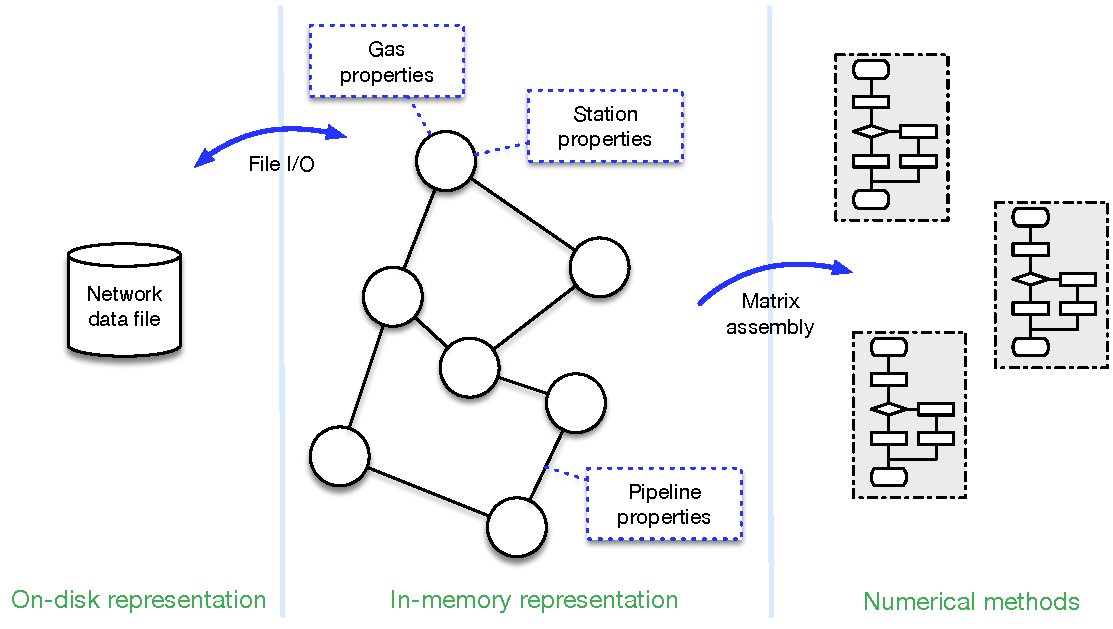
\includegraphics[scale = 0.4]{img_intro/system_arch.pdf}
    \begin{tikzpicture}
    \node[anchor=south west,inner sep=0] (X) at (2, -3) 
    {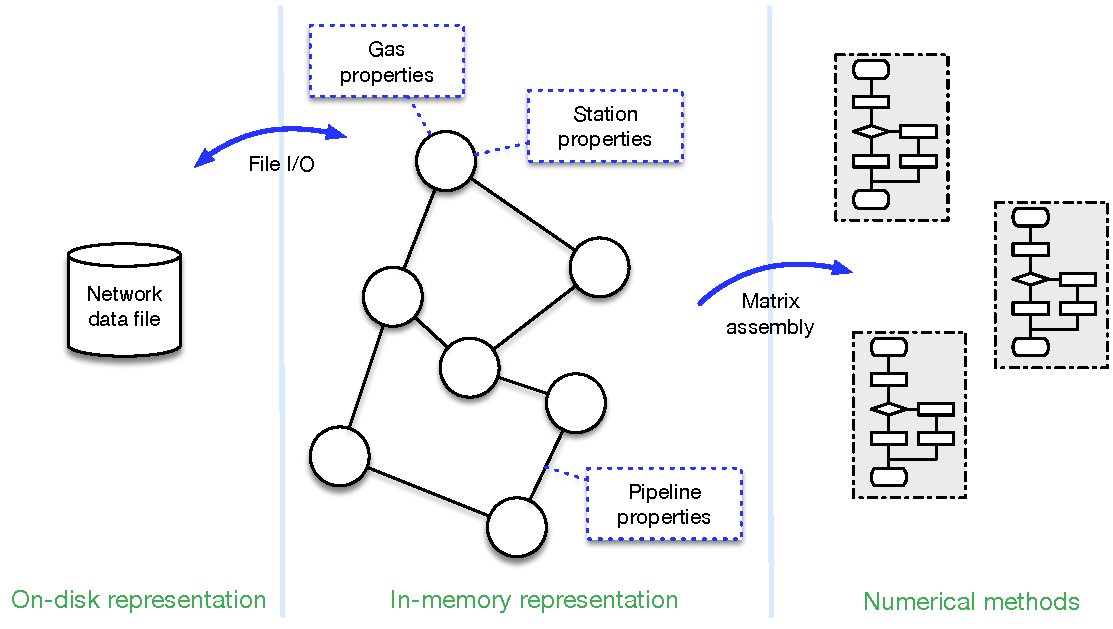
\includegraphics[scale = 0.5]{img_intro/system_arch.pdf}};
    \node [blue, ultra thick] at ($(X.south west)!0.5!(X.north east)$) {};
    % Square for scale 0.4
    %\draw[red] (9.75,-3) -- (9.75,1.25) -- (4.0,1.25) -- (4.0,-3) -- cycle;
    % Square for scale 0.5
    \draw[red] (11.75,-3) -- (11.75,2.25) -- (4.5,2.25) -- (4.5,-3) -- cycle;
    \pgfsetfillcolor{vinotinto}
    \pgfsetfillopacity{0.25}
    \only<2>\fill(8.5,-3) -- (8.5,2.25) -- (4.5,2.25) -- (4.5,-3) -- cycle;
    \only<3>\fill(8.5,-3) -- (8.5,2.25) -- (11.75,2.25) -- (11.75,-3) -- cycle;
    
    \end{tikzpicture}
    \caption{Taken from architecture proposal (Matteo's presentation).}
\end{figure}
   
\end{frame}

%----------------------------------------------------------------
%----------------------------------------------------------------

\begin{frame}{Numerical methods stage}
\noindent
%\psframe[fillstyle=solid,fillcolor=blue!20,linewidth=3pt,linecolor=black](0,0)(21,16)


\begin{minipage}{0.25\textwidth}
% Graphic for TeX using PGF
% Title: /home/karol/Documents/UNIVERSITA/POLITO/PRESENTATIONS/SHIMMER_2024_01/img_code/numerical_methods_algorithm.dia
% Creator: Dia v0.97.3
% CreationDate: Mon Jan 22 14:41:21 2024
% For: karol
% \usepackage{tikz}
% The following commands are not supported in PSTricks at present
% We define them conditionally, so when they are implemented,
% this pgf file will use them.
\ifx\du\undefined
  \newlength{\du}
\fi
\setlength{\du}{7.5\unitlength}
\begin{tikzpicture}[even odd rule]
\pgftransformxscale{1.000000}
\pgftransformyscale{-1.000000}
\definecolor{dialinecolor}{rgb}{0.000000, 0.000000, 0.000000}
\pgfsetstrokecolor{dialinecolor}
\pgfsetstrokeopacity{1.000000}
\definecolor{diafillcolor}{rgb}{1.000000, 1.000000, 1.000000}
\pgfsetfillcolor{diafillcolor}
\pgfsetfillopacity{1.000000}
\pgfsetlinewidth{0.100000\du}
\pgfsetdash{{\pgflinewidth}{0.200000\du}}{0cm}
\pgfsetmiterjoin
\pgfsetbuttcap
{
%\pgfsetcornersarced{\pgfpoint{0.000000\du}{0.000000\du}}\definecolor{diafillcolor}{rgb}{0.898039, 0.898039, 0.898039}
\pgfsetcornersarced{\pgfpoint{0.000000\du}{0.000000\du}}
\pgfsetfillcolor{lgreyblue}
\pgfsetfillopacity{1.000000}
\fill (5.263771\du,-6.474566\du)--(5.263771\du,15.452514\du)--(19.576450\du,15.452514\du)--(19.576450\du,-6.474566\du)--cycle;
}{\pgfsetcornersarced{\pgfpoint{0.000000\du}{0.000000\du}}\definecolor{dialinecolor}{rgb}{0.000000, 0.000000, 0.000000}
% Time stroke
\only<1-2>{\pgfsetstrokecolor{diafillcolor}}
\only<3->{\pgfsetstrokecolor{red}}

\pgfsetstrokeopacity{1.000000}
\draw (5.263771\du,-6.474566\du)--(5.263771\du,15.452514\du)--(19.576450\du,15.452514\du)--(19.576450\du,-6.474566\du)--cycle;
}\pgfsetlinewidth{0.100000\du}
\pgfsetdash{{\pgflinewidth}{0.200000\du}}{0cm}
\pgfsetmiterjoin
\pgfsetbuttcap
{\pgfsetcornersarced{\pgfpoint{0.000000\du}{0.000000\du}}\definecolor{diafillcolor}{rgb}{0.945098, 0.882353, 0.921569}
\pgfsetfillcolor{diafillcolor}
\pgfsetfillopacity{1.000000}
\fill (6.382560\du,-3.393932\du)--(6.382560\du,10.487096\du)--(17.858929\du,10.487096\du)--(17.858929\du,-3.393932\du)--cycle;
}{\pgfsetcornersarced{\pgfpoint{0.000000\du}{0.000000\du}}\definecolor{dialinecolor}{rgb}{0.403922, 0.047059, 0.274510}
\only<1>{\pgfsetstrokecolor{dialinecolor}}
\only<2->{\pgfsetstrokecolor{red}}
\pgfsetstrokeopacity{1.000000}
\draw (6.382560\du,-3.393932\du)--(6.382560\du,10.487096\du)--(17.858929\du,10.487096\du)--(17.858929\du,-3.393932\du)--cycle;
}\pgfsetlinewidth{0.100000\du}
\pgfsetdash{{\pgflinewidth}{0.200000\du}}{0cm}
\pgfsetmiterjoin
\pgfsetbuttcap
{\pgfsetcornersarced{\pgfpoint{0.000000\du}{0.000000\du}}\definecolor{diafillcolor}{rgb}{0.847059, 0.898039, 0.898039}
\pgfsetfillcolor{diafillcolor}
\pgfsetfillopacity{1.000000}
\fill (7.111444\du,-0.032868\du)--(7.111444\du,7.295393\du)--(13.953260\du,7.295393\du)--(13.953260\du,-0.032868\du)--cycle;
}{\pgfsetcornersarced{\pgfpoint{0.000000\du}{0.000000\du}}\definecolor{dialinecolor}{rgb}{0.003876, 0.318700, 0.318700}
\pgfsetstrokecolor{dialinecolor}
\pgfsetstrokeopacity{1.000000}
\draw (7.111444\du,-0.032868\du)--(7.111444\du,7.295393\du)--(13.953260\du,7.295393\du)--(13.953260\du,-0.032868\du)--cycle;
}\pgfsetlinewidth{0.100000\du}
\pgfsetdash{}{0pt}
\pgfsetbuttcap
\pgfsetmiterjoin
\pgfsetlinewidth{0.100000\du}
\pgfsetbuttcap
\pgfsetmiterjoin
\pgfsetdash{}{0pt}
\definecolor{diafillcolor}{rgb}{1.000000, 1.000000, 1.000000}
\pgfsetfillcolor{diafillcolor}
\pgfsetfillopacity{1.000000}
\definecolor{dialinecolor}{rgb}{0.000000, 0.000000, 0.000000}
\pgfsetstrokecolor{dialinecolor}
\pgfsetstrokeopacity{1.000000}
\pgfpathmoveto{\pgfpoint{8.300000\du}{0.200000\du}}
\pgfpathlineto{\pgfpoint{9.900000\du}{0.200000\du}}
\pgfpathcurveto{\pgfpoint{10.120914\du}{0.200000\du}}{\pgfpoint{10.300000\du}{0.401472\du}}{\pgfpoint{10.300000\du}{0.650000\du}}
\pgfpathcurveto{\pgfpoint{10.300000\du}{0.898528\du}}{\pgfpoint{10.120914\du}{1.100000\du}}{\pgfpoint{9.900000\du}{1.100000\du}}
\pgfpathlineto{\pgfpoint{8.300000\du}{1.100000\du}}
\pgfpathcurveto{\pgfpoint{8.079086\du}{1.100000\du}}{\pgfpoint{7.900000\du}{0.898528\du}}{\pgfpoint{7.900000\du}{0.650000\du}}
\pgfpathcurveto{\pgfpoint{7.900000\du}{0.401472\du}}{\pgfpoint{8.079086\du}{0.200000\du}}{\pgfpoint{8.300000\du}{0.200000\du}}
\pgfpathclose
\pgfusepath{fill,stroke}
% setfont left to latex
% setfont left to latex
\definecolor{dialinecolor}{rgb}{0.000000, 0.000000, 0.000000}
\pgfsetstrokecolor{dialinecolor}
\pgfsetstrokeopacity{1.000000}
\definecolor{diafillcolor}{rgb}{0.000000, 0.000000, 0.000000}
\pgfsetfillcolor{diafillcolor}
\pgfsetfillopacity{1.000000}
\node[anchor=base,inner sep=0pt, outer sep=0pt,color=dialinecolor] at (9.100000\du,0.950000\du){};
\pgfsetlinewidth{0.100000\du}
\pgfsetdash{}{0pt}
\pgfsetbuttcap
{
\definecolor{diafillcolor}{rgb}{0.000000, 0.000000, 0.000000}
\pgfsetfillcolor{diafillcolor}
\pgfsetfillopacity{1.000000}
% was here!!!
\definecolor{dialinecolor}{rgb}{0.000000, 0.000000, 0.000000}
\pgfsetstrokecolor{dialinecolor}
\pgfsetstrokeopacity{1.000000}
\draw (9.100000\du,1.100000\du)--(9.100000\du,1.550000\du);
}
\pgfsetlinewidth{0.100000\du}
\pgfsetdash{}{0pt}
\pgfsetmiterjoin
{\pgfsetcornersarced{\pgfpoint{0.000000\du}{0.000000\du}}\definecolor{diafillcolor}{rgb}{1.000000, 1.000000, 1.000000}
\pgfsetfillcolor{diafillcolor}
\pgfsetfillopacity{1.000000}
\fill (7.600000\du,1.550000\du)--(7.600000\du,2.323485\du)--(10.600000\du,2.323485\du)--(10.600000\du,1.550000\du)--cycle;
}{\pgfsetcornersarced{\pgfpoint{0.000000\du}{0.000000\du}}\definecolor{dialinecolor}{rgb}{0.000000, 0.000000, 0.000000}
\pgfsetstrokecolor{dialinecolor}
\pgfsetstrokeopacity{1.000000}
\draw (7.600000\du,1.550000\du)--(7.600000\du,2.323485\du)--(10.600000\du,2.323485\du)--(10.600000\du,1.550000\du)--cycle;
}% setfont left to latex
% setfont left to latex
\definecolor{dialinecolor}{rgb}{0.000000, 0.000000, 0.000000}
\pgfsetstrokecolor{dialinecolor}
\pgfsetstrokeopacity{1.000000}
\definecolor{diafillcolor}{rgb}{0.000000, 0.000000, 0.000000}
\pgfsetfillcolor{diafillcolor}
\pgfsetfillopacity{1.000000}
\node[anchor=base,inner sep=0pt, outer sep=0pt,color=dialinecolor] at (9.100000\du,2.191526\du){};
\pgfsetlinewidth{0.100000\du}
\pgfsetdash{}{0pt}
\pgfsetmiterjoin
\definecolor{diafillcolor}{rgb}{1.000000, 1.000000, 1.000000}
\pgfsetfillcolor{diafillcolor}
\pgfsetfillopacity{1.000000}
\fill (9.099017\du,2.996875\du)--(10.616784\du,3.496875\du)--(9.099017\du,3.996875\du)--(7.581250\du,3.496875\du)--cycle;
\definecolor{dialinecolor}{rgb}{0.000000, 0.000000, 0.000000}
\pgfsetstrokecolor{dialinecolor}
\pgfsetstrokeopacity{1.000000}
\draw (9.099017\du,2.996875\du)--(10.616784\du,3.496875\du)--(9.099017\du,3.996875\du)--(7.581250\du,3.496875\du)--cycle;
% setfont left to latex
% setfont left to latex
\definecolor{dialinecolor}{rgb}{0.000000, 0.000000, 0.000000}
\pgfsetstrokecolor{dialinecolor}
\pgfsetstrokeopacity{1.000000}
\definecolor{diafillcolor}{rgb}{0.000000, 0.000000, 0.000000}
\pgfsetfillcolor{diafillcolor}
\pgfsetfillopacity{1.000000}
\node[anchor=base,inner sep=0pt, outer sep=0pt,color=dialinecolor] at (9.099017\du,3.781875\du){};
\pgfsetlinewidth{0.100000\du}
\pgfsetdash{}{0pt}
\pgfsetbuttcap
{
\definecolor{diafillcolor}{rgb}{0.000000, 0.000000, 0.000000}
\pgfsetfillcolor{diafillcolor}
\pgfsetfillopacity{1.000000}
% was here!!!
\definecolor{dialinecolor}{rgb}{0.000000, 0.000000, 0.000000}
\pgfsetstrokecolor{dialinecolor}
\pgfsetstrokeopacity{1.000000}
\draw (9.099017\du,3.996875\du)--(9.102774\du,4.529549\du);
}
\pgfsetlinewidth{0.100000\du}
\pgfsetdash{}{0pt}
\pgfsetmiterjoin
{\pgfsetcornersarced{\pgfpoint{0.000000\du}{0.000000\du}}\definecolor{diafillcolor}{rgb}{1.000000, 1.000000, 1.000000}
\pgfsetfillcolor{diafillcolor}
\pgfsetfillopacity{1.000000}
\fill (7.602774\du,4.529549\du)--(7.602774\du,5.346335\du)--(10.602774\du,5.346335\du)--(10.602774\du,4.529549\du)--cycle;
}{\pgfsetcornersarced{\pgfpoint{0.000000\du}{0.000000\du}}\definecolor{dialinecolor}{rgb}{0.000000, 0.000000, 0.000000}
\pgfsetstrokecolor{dialinecolor}
\pgfsetstrokeopacity{1.000000}
\draw (7.602774\du,4.529549\du)--(7.602774\du,5.346335\du)--(10.602774\du,5.346335\du)--(10.602774\du,4.529549\du)--cycle;
}% setfont left to latex
% setfont left to latex
\definecolor{dialinecolor}{rgb}{0.000000, 0.000000, 0.000000}
\pgfsetstrokecolor{dialinecolor}
\pgfsetstrokeopacity{1.000000}
\definecolor{diafillcolor}{rgb}{0.000000, 0.000000, 0.000000}
\pgfsetfillcolor{diafillcolor}
\pgfsetfillopacity{1.000000}
\node[anchor=base,inner sep=0pt, outer sep=0pt,color=dialinecolor] at (9.102774\du,5.192725\du){};
\pgfsetlinewidth{0.100000\du}
\pgfsetdash{}{0pt}
\pgfsetbuttcap
{
\definecolor{diafillcolor}{rgb}{0.000000, 0.000000, 0.000000}
\pgfsetfillcolor{diafillcolor}
\pgfsetfillopacity{1.000000}
% was here!!!
\definecolor{dialinecolor}{rgb}{0.000000, 0.000000, 0.000000}
\pgfsetstrokecolor{dialinecolor}
\pgfsetstrokeopacity{1.000000}
\draw (9.100000\du,2.323485\du)--(9.099017\du,2.996875\du);
}
\pgfsetlinewidth{0.100000\du}
\pgfsetdash{}{0pt}
\pgfsetbuttcap
{
\definecolor{diafillcolor}{rgb}{0.000000, 0.000000, 0.000000}
\pgfsetfillcolor{diafillcolor}
\pgfsetfillopacity{1.000000}
% was here!!!
\definecolor{dialinecolor}{rgb}{0.000000, 0.000000, 0.000000}
\pgfsetstrokecolor{dialinecolor}
\pgfsetstrokeopacity{1.000000}
\draw (10.616784\du,3.496875\du)--(11.080431\du,3.494330\du);
}
\pgfsetlinewidth{0.100000\du}
\pgfsetdash{}{0pt}
\pgfsetmiterjoin
{\pgfsetcornersarced{\pgfpoint{0.000000\du}{0.000000\du}}\definecolor{diafillcolor}{rgb}{1.000000, 1.000000, 1.000000}
\pgfsetfillcolor{diafillcolor}
\pgfsetfillopacity{1.000000}
\fill (11.080431\du,3.085936\du)--(11.080431\du,3.902723\du)--(13.643775\du,3.902723\du)--(13.643775\du,3.085936\du)--cycle;
}{\pgfsetcornersarced{\pgfpoint{0.000000\du}{0.000000\du}}\definecolor{dialinecolor}{rgb}{0.000000, 0.000000, 0.000000}
\pgfsetstrokecolor{dialinecolor}
\pgfsetstrokeopacity{1.000000}
\draw (11.080431\du,3.085936\du)--(11.080431\du,3.902723\du)--(13.643775\du,3.902723\du)--(13.643775\du,3.085936\du)--cycle;
}% setfont left to latex
% setfont left to latex
\definecolor{dialinecolor}{rgb}{0.000000, 0.000000, 0.000000}
\pgfsetstrokecolor{dialinecolor}
\pgfsetstrokeopacity{1.000000}
\definecolor{diafillcolor}{rgb}{0.000000, 0.000000, 0.000000}
\pgfsetfillcolor{diafillcolor}
\pgfsetfillopacity{1.000000}
\node[anchor=base,inner sep=0pt, outer sep=0pt,color=dialinecolor] at (12.362103\du,3.749113\du){};
\pgfsetlinewidth{0.100000\du}
\pgfsetdash{}{0pt}
\pgfsetmiterjoin
\pgfsetbuttcap
{
\definecolor{diafillcolor}{rgb}{0.000000, 0.000000, 0.000000}
\pgfsetfillcolor{diafillcolor}
\pgfsetfillopacity{1.000000}
% was here!!!
{\pgfsetcornersarced{\pgfpoint{0.000000\du}{0.000000\du}}\definecolor{dialinecolor}{rgb}{0.000000, 0.000000, 0.000000}
\pgfsetstrokecolor{dialinecolor}
\pgfsetstrokeopacity{1.000000}
\draw (10.602774\du,5.142139\du)--(12.362103\du,5.142139\du)--(12.362103\du,3.902723\du);
}}
\pgfsetlinewidth{0.100000\du}
\pgfsetdash{}{0pt}
\pgfsetbuttcap
\pgfsetmiterjoin
\pgfsetlinewidth{0.100000\du}
\pgfsetbuttcap
\pgfsetmiterjoin
\pgfsetdash{}{0pt}
\definecolor{diafillcolor}{rgb}{1.000000, 1.000000, 1.000000}
\pgfsetfillcolor{diafillcolor}
\pgfsetfillopacity{1.000000}
\definecolor{dialinecolor}{rgb}{0.000000, 0.000000, 0.000000}
\pgfsetstrokecolor{dialinecolor}
\pgfsetstrokeopacity{1.000000}
\pgfpathmoveto{\pgfpoint{8.304290\du}{5.979312\du}}
\pgfpathlineto{\pgfpoint{9.904290\du}{5.979312\du}}
\pgfpathcurveto{\pgfpoint{10.125204\du}{5.979312\du}}{\pgfpoint{10.304290\du}{6.180783\du}}{\pgfpoint{10.304290\du}{6.429312\du}}
\pgfpathcurveto{\pgfpoint{10.304290\du}{6.677840\du}}{\pgfpoint{10.125204\du}{6.879312\du}}{\pgfpoint{9.904290\du}{6.879312\du}}
\pgfpathlineto{\pgfpoint{8.304290\du}{6.879312\du}}
\pgfpathcurveto{\pgfpoint{8.083376\du}{6.879312\du}}{\pgfpoint{7.904290\du}{6.677840\du}}{\pgfpoint{7.904290\du}{6.429312\du}}
\pgfpathcurveto{\pgfpoint{7.904290\du}{6.180783\du}}{\pgfpoint{8.083376\du}{5.979312\du}}{\pgfpoint{8.304290\du}{5.979312\du}}
\pgfpathclose
\pgfusepath{fill,stroke}
% setfont left to latex
% setfont left to latex
\definecolor{dialinecolor}{rgb}{0.000000, 0.000000, 0.000000}
\pgfsetstrokecolor{dialinecolor}
\pgfsetstrokeopacity{1.000000}
\definecolor{diafillcolor}{rgb}{0.000000, 0.000000, 0.000000}
\pgfsetfillcolor{diafillcolor}
\pgfsetfillopacity{1.000000}
\node[anchor=base,inner sep=0pt, outer sep=0pt,color=dialinecolor] at (9.104290\du,6.729312\du){};
\pgfsetlinewidth{0.100000\du}
\pgfsetdash{}{0pt}
\pgfsetbuttcap
{
\definecolor{diafillcolor}{rgb}{0.000000, 0.000000, 0.000000}
\pgfsetfillcolor{diafillcolor}
\pgfsetfillopacity{1.000000}
% was here!!!
\definecolor{dialinecolor}{rgb}{0.000000, 0.000000, 0.000000}
\pgfsetstrokecolor{dialinecolor}
\pgfsetstrokeopacity{1.000000}
\draw (9.102774\du,5.346335\du)--(9.104290\du,5.979312\du);
}
% setfont left to latex
% setfont left to latex
\definecolor{dialinecolor}{rgb}{0.000000, 0.000000, 0.000000}
\pgfsetstrokecolor{dialinecolor}
\pgfsetstrokeopacity{1.000000}
\definecolor{diafillcolor}{rgb}{0.000000, 0.000000, 0.000000}
\pgfsetfillcolor{diafillcolor}
\pgfsetfillopacity{1.000000}
\node[anchor=base west,inner sep=0pt,outer sep=0pt,color=dialinecolor] at (11.506559\du,-0.738088\du){};
% setfont left to latex
% setfont left to latex

\pgfsetstrokecolor{dialinecolor}
\pgfsetstrokeopacity{1.000000}
\pgfsetfillcolor{diafillcolor}
\pgfsetfillopacity{1.000000}
\node[anchor=base west,inner sep=0pt,outer sep=0pt,color=tealgreen] at (11.5\du,0.8 \du){\scriptsize {\textbf{Fluid}}};
\node[anchor=base west,inner sep=0pt,outer sep=0pt,color=tealgreen] at (11.5\du,1.55\du){\scriptsize {\textbf{solver}}};


\definecolor{dialinecolor}{rgb}{0.000000, 0.317647, 0.317647}
\pgfsetstrokecolor{dialinecolor}
\pgfsetstrokeopacity{1.000000}
\definecolor{diafillcolor}{rgb}{0.000000, 0.317647, 0.317647}
\pgfsetfillcolor{red}
\pgfsetfillopacity{1.000000}
% setfont left to latex
% setfont left to latex
\definecolor{dialinecolor}{rgb}{0.000000, 0.317647, 0.317647}
\pgfsetstrokecolor{dialinecolor}
\pgfsetstrokeopacity{1.000000}
\definecolor{diafillcolor}{rgb}{0.000000, 0.317647, 0.317647}
\pgfsetfillcolor{red}
\pgfsetfillopacity{1.000000}
\node[anchor=base west,inner sep=0pt,outer sep=0pt,color=dialinecolor] at (11.178222\du,1.315313\du){};
% setfont left to latex
% setfont left to latex
\definecolor{dialinecolor}{rgb}{0.000000, 0.000000, 0.000000}
\pgfsetstrokecolor{dialinecolor}
\pgfsetstrokeopacity{1.000000}
\definecolor{diafillcolor}{rgb}{0.000000, 0.000000, 0.000000}
\pgfsetfillcolor{diafillcolor}
\pgfsetfillopacity{1.000000}
\node[anchor=base west,inner sep=0pt,outer sep=0pt,color=dialinecolor] at (9.691002\du,-1.143346\du){};
% setfont left to latex
% setfont left to latex
\definecolor{dialinecolor}{rgb}{0.000000, 0.000000, 0.000000}
\pgfsetstrokecolor{dialinecolor}
\pgfsetstrokeopacity{1.000000}
\definecolor{diafillcolor}{rgb}{0.000000, 0.000000, 0.000000}
\pgfsetfillcolor{diafillcolor}
\pgfsetfillopacity{1.000000}
\node[anchor=base west,inner sep=0pt,outer sep=0pt,color=dialinecolor] at (9.766373\du,10.513799\du){};
% setfont left to latex
% setfont left to latex

\pgfsetstrokecolor{red}
\pgfsetstrokeopacity{1.000000}

\only<1>{\node[anchor=base west,inner sep=0pt,outer sep=0pt,color=vinotinto] at (11\du,-1.5\du){\scriptsize \textbf{Quality cycle}}};
\only<2->{\node[anchor=base west,inner sep=0pt,outer sep=0pt,color=red] at (11\du,-1.5\du){\scriptsize \textbf{Quality cycle}};}
\pgfsetlinewidth{0.100000\du}
\pgfsetdash{}{0pt}
\pgfsetbuttcap
{
\definecolor{diafillcolor}{rgb}{0.000000, 0.000000, 0.000000}
\pgfsetfillcolor{diafillcolor}
\pgfsetfillopacity{1.000000}
% was here!!!
\definecolor{dialinecolor}{rgb}{0.000000, 0.000000, 0.000000}
\pgfsetstrokecolor{dialinecolor}
\pgfsetstrokeopacity{1.000000}
\draw (9.099526\du,6.929167\du)--(9.090757\du,7.849149\du);
}
\pgfsetlinewidth{0.100000\du}
\pgfsetdash{}{0pt}
\pgfsetmiterjoin
{\pgfsetcornersarced{\pgfpoint{0.000000\du}{0.000000\du}}\definecolor{diafillcolor}{rgb}{1.000000, 1.000000, 1.000000}
\pgfsetfillcolor{diafillcolor}
\pgfsetfillopacity{1.000000}
\fill (7.590757\du,7.849149\du)--(7.590757\du,8.622634\du)--(10.590757\du,8.622634\du)--(10.590757\du,7.849149\du)--cycle;
}{\pgfsetcornersarced{\pgfpoint{0.000000\du}{0.000000\du}}\definecolor{dialinecolor}{rgb}{0.000000, 0.000000, 0.000000}
\pgfsetstrokecolor{dialinecolor}
\pgfsetstrokeopacity{1.000000}
\draw (7.590757\du,7.849149\du)--(7.590757\du,8.622634\du)--(10.590757\du,8.622634\du)--(10.590757\du,7.849149\du)--cycle;
}% setfont left to latex
% setfont left to latex
\definecolor{dialinecolor}{rgb}{0.000000, 0.000000, 0.000000}
\pgfsetstrokecolor{dialinecolor}
\pgfsetstrokeopacity{1.000000}
\definecolor{diafillcolor}{rgb}{0.000000, 0.000000, 0.000000}
\pgfsetfillcolor{diafillcolor}
\pgfsetfillopacity{1.000000}
\node[anchor=base,inner sep=0pt, outer sep=0pt,color=dialinecolor] at (9.090757\du,8.490675\du){};
\pgfsetlinewidth{0.100000\du}
\pgfsetdash{}{0pt}
\pgfsetmiterjoin
\definecolor{diafillcolor}{rgb}{1.000000, 1.000000, 1.000000}
\pgfsetfillcolor{diafillcolor}
\pgfsetfillopacity{1.000000}
\fill (9.089775\du,8.996139\du)--(10.607542\du,9.496139\du)--(9.089775\du,9.996139\du)--(7.572008\du,9.496139\du)--cycle;
\definecolor{dialinecolor}{rgb}{0.000000, 0.000000, 0.000000}
\pgfsetstrokecolor{dialinecolor}
\pgfsetstrokeopacity{1.000000}
\draw (9.089775\du,8.996139\du)--(10.607542\du,9.496139\du)--(9.089775\du,9.996139\du)--(7.572008\du,9.496139\du)--cycle;
% setfont left to latex
% setfont left to latex
\definecolor{dialinecolor}{rgb}{0.000000, 0.000000, 0.000000}
\pgfsetstrokecolor{dialinecolor}
\pgfsetstrokeopacity{1.000000}
\definecolor{diafillcolor}{rgb}{0.000000, 0.000000, 0.000000}
\pgfsetfillcolor{diafillcolor}
\pgfsetfillopacity{1.000000}
\node[anchor=base,inner sep=0pt, outer sep=0pt,color=dialinecolor] at (9.089775\du,9.781139\du){};
\pgfsetlinewidth{0.100000\du}
\pgfsetdash{}{0pt}
\pgfsetbuttcap
{
\definecolor{diafillcolor}{rgb}{0.000000, 0.000000, 0.000000}
\pgfsetfillcolor{diafillcolor}
\pgfsetfillopacity{1.000000}
% was here!!!
\definecolor{dialinecolor}{rgb}{0.000000, 0.000000, 0.000000}
\pgfsetstrokecolor{dialinecolor}
\pgfsetstrokeopacity{1.000000}
\draw (9.090757\du,8.622634\du)--(9.089775\du,8.996139\du);
}
\pgfsetlinewidth{0.100000\du}
\pgfsetdash{}{0pt}
\pgfsetmiterjoin
{\pgfsetcornersarced{\pgfpoint{0.000000\du}{0.000000\du}}\definecolor{diafillcolor}{rgb}{1.000000, 1.000000, 1.000000}
\pgfsetfillcolor{diafillcolor}
\pgfsetfillopacity{1.000000}
\fill (14.966081\du,7.491214\du)--(14.966081\du,8.308000\du)--(17.529425\du,8.308000\du)--(17.529425\du,7.491214\du)--cycle;
}{\pgfsetcornersarced{\pgfpoint{0.000000\du}{0.000000\du}}\definecolor{dialinecolor}{rgb}{0.000000, 0.000000, 0.000000}
\pgfsetstrokecolor{dialinecolor}
\pgfsetstrokeopacity{1.000000}
\draw (14.966081\du,7.491214\du)--(14.966081\du,8.308000\du)--(17.529425\du,8.308000\du)--(17.529425\du,7.491214\du)--cycle;
}% setfont left to latex
% setfont left to latex
\definecolor{dialinecolor}{rgb}{0.000000, 0.000000, 0.000000}
\pgfsetstrokecolor{dialinecolor}
\pgfsetstrokeopacity{1.000000}
\definecolor{diafillcolor}{rgb}{0.000000, 0.000000, 0.000000}
\pgfsetfillcolor{diafillcolor}
\pgfsetfillopacity{1.000000}
\node[anchor=base,inner sep=0pt, outer sep=0pt,color=dialinecolor] at (16.247753\du,8.154390\du){};
\pgfsetlinewidth{0.100000\du}
\pgfsetdash{}{0pt}
\pgfsetmiterjoin
\pgfsetbuttcap
{
\definecolor{diafillcolor}{rgb}{0.000000, 0.000000, 0.000000}
\pgfsetfillcolor{diafillcolor}
\pgfsetfillopacity{1.000000}
% was here!!!
{\pgfsetcornersarced{\pgfpoint{0.000000\du}{0.000000\du}}\definecolor{dialinecolor}{rgb}{0.000000, 0.000000, 0.000000}
\pgfsetstrokecolor{dialinecolor}
\pgfsetstrokeopacity{1.000000}
\draw (10.607542\du,9.496139\du)--(16.250456\du,9.496139\du)--(16.250456\du,8.308000\du)--(16.247753\du,8.308000\du);
}}
\pgfsetlinewidth{0.100000\du}
\pgfsetdash{}{0pt}
\pgfsetmiterjoin
\pgfsetbuttcap
{
\definecolor{diafillcolor}{rgb}{0.000000, 0.000000, 0.000000}
\pgfsetfillcolor{diafillcolor}
\pgfsetfillopacity{1.000000}
% was here!!!
{\pgfsetcornersarced{\pgfpoint{0.000000\du}{0.000000\du}}\definecolor{dialinecolor}{rgb}{0.000000, 0.000000, 0.000000}
\pgfsetstrokecolor{dialinecolor}
\pgfsetstrokeopacity{1.000000}
\draw (16.247753\du,7.491214\du)--(16.247753\du,-1.240844\du)--(10.609252\du,-1.240844\du)--(10.609252\du,-1.258752\du);
}}
\pgfsetlinewidth{0.100000\du}
\pgfsetdash{}{0pt}
\pgfsetbuttcap
{
\definecolor{diafillcolor}{rgb}{0.000000, 0.000000, 0.000000}
\pgfsetfillcolor{diafillcolor}
\pgfsetfillopacity{1.000000}
% was here!!!
\definecolor{dialinecolor}{rgb}{0.000000, 0.000000, 0.000000}
\pgfsetstrokecolor{dialinecolor}
\pgfsetstrokeopacity{1.000000}
\draw (9.089775\du,9.996139\du)--(9.078930\du,11.105818\du);
}
\pgfsetlinewidth{0.100000\du}
\pgfsetdash{}{0pt}
\pgfsetmiterjoin
{\pgfsetcornersarced{\pgfpoint{0.000000\du}{0.000000\du}}\definecolor{diafillcolor}{rgb}{1.000000, 1.000000, 1.000000}
\pgfsetfillcolor{diafillcolor}
\pgfsetfillopacity{1.000000}
\fill (7.578930\du,11.105818\du)--(7.578930\du,11.879303\du)--(10.578930\du,11.879303\du)--(10.578930\du,11.105818\du)--cycle;
}{\pgfsetcornersarced{\pgfpoint{0.000000\du}{0.000000\du}}\definecolor{dialinecolor}{rgb}{0.000000, 0.000000, 0.000000}
\pgfsetstrokecolor{dialinecolor}
\pgfsetstrokeopacity{1.000000}
\draw (7.578930\du,11.105818\du)--(7.578930\du,11.879303\du)--(10.578930\du,11.879303\du)--(10.578930\du,11.105818\du)--cycle;
}% setfont left to latex
% setfont left to latex
\definecolor{dialinecolor}{rgb}{0.000000, 0.000000, 0.000000}
\pgfsetstrokecolor{dialinecolor}
\pgfsetstrokeopacity{1.000000}
\definecolor{diafillcolor}{rgb}{0.000000, 0.000000, 0.000000}
\pgfsetfillcolor{diafillcolor}
\pgfsetfillopacity{1.000000}
\node[anchor=base,inner sep=0pt, outer sep=0pt,color=dialinecolor] at (9.078930\du,11.747344\du){};
\pgfsetlinewidth{0.100000\du}
\pgfsetdash{}{0pt}
\pgfsetmiterjoin
\definecolor{diafillcolor}{rgb}{1.000000, 1.000000, 1.000000}
\pgfsetfillcolor{diafillcolor}
\pgfsetfillopacity{1.000000}
\fill (9.077947\du,12.443644\du)--(10.595714\du,12.943644\du)--(9.077947\du,13.443644\du)--(7.560180\du,12.943644\du)--cycle;
\definecolor{dialinecolor}{rgb}{0.000000, 0.000000, 0.000000}
\pgfsetstrokecolor{dialinecolor}
\pgfsetstrokeopacity{1.000000}
\draw (9.077947\du,12.443644\du)--(10.595714\du,12.943644\du)--(9.077947\du,13.443644\du)--(7.560180\du,12.943644\du)--cycle;
% setfont left to latex
% setfont left to latex
\definecolor{dialinecolor}{rgb}{0.000000, 0.000000, 0.000000}
\pgfsetstrokecolor{dialinecolor}
\pgfsetstrokeopacity{1.000000}
\definecolor{diafillcolor}{rgb}{0.000000, 0.000000, 0.000000}
\pgfsetfillcolor{diafillcolor}
\pgfsetfillopacity{1.000000}
\node[anchor=base,inner sep=0pt, outer sep=0pt,color=dialinecolor] at (9.077947\du,13.228644\du){};
\pgfsetlinewidth{0.100000\du}
\pgfsetdash{}{0pt}
\pgfsetbuttcap
{
\definecolor{diafillcolor}{rgb}{0.000000, 0.000000, 0.000000}
\pgfsetfillcolor{diafillcolor}
\pgfsetfillopacity{1.000000}
% was here!!!
\definecolor{dialinecolor}{rgb}{0.000000, 0.000000, 0.000000}
\pgfsetstrokecolor{dialinecolor}
\pgfsetstrokeopacity{1.000000}
\draw (9.078930\du,11.879303\du)--(9.077947\du,12.443644\du);
}
\pgfsetlinewidth{0.100000\du}
\pgfsetdash{}{0pt}
\pgfsetmiterjoin
{\pgfsetcornersarced{\pgfpoint{0.000000\du}{0.000000\du}}
\definecolor{diafillcolor}{rgb}{1.000000, 1.000000, 1.000000}
\pgfsetfillcolor{diafillcolor}
\pgfsetfillopacity{1.000000}
\fill (14.790680\du,12.574453\du)--(14.790680\du,13.391240\du)--(17.354023\du,13.391240\du)--(17.354023\du,12.574453\du)--cycle;
}{\pgfsetcornersarced{\pgfpoint{0.000000\du}{0.000000\du}}\definecolor{dialinecolor}{rgb}{0.000000, 0.000000, 0.000000}
\pgfsetstrokecolor{dialinecolor}
\pgfsetstrokeopacity{1.000000}
\draw (14.790680\du,12.574453\du)--(14.790680\du,13.391240\du)--(17.354023\du,13.391240\du)--(17.354023\du,12.574453\du)--cycle;
}% setfont left to latex
% setfont left to latex
\definecolor{dialinecolor}{rgb}{0.000000, 0.000000, 0.000000}
\pgfsetstrokecolor{dialinecolor}
\pgfsetstrokeopacity{1.000000}
\definecolor{diafillcolor}{rgb}{0.000000, 0.000000, 0.000000}
\pgfsetfillcolor{diafillcolor}
\pgfsetfillopacity{1.000000}
\node[anchor=base,inner sep=0pt, outer sep=0pt,color=dialinecolor] at (16.072352\du,13.237630\du){};
\pgfsetlinewidth{0.100000\du}
\pgfsetdash{}{0pt}
\pgfsetmiterjoin
% Quality square
{\pgfsetcornersarced{\pgfpoint{0.000000\du}{0.000000\du}}\definecolor{diafillcolor}{rgb}{1.000000, 1.000000, 1.000000}
\pgfsetfillcolor{diafillcolor}
\pgfsetfillopacity{1.000000}
\fill (7.609252\du,-1.645494\du)--(7.609252\du,-0.872009\du)--(10.609252\du,-0.872009\du)--(10.609252\du,-1.645494\du)--cycle;
}{\pgfsetcornersarced{\pgfpoint{0.000000\du}{0.000000\du}}\definecolor{dialinecolor}{rgb}{0.000000, 0.000000, 0.000000}
\pgfsetstrokecolor{dialinecolor}
\pgfsetstrokeopacity{1.000000}
\draw (7.609252\du,-1.645494\du)--(7.609252\du,-0.872009\du)--(10.609252\du,-0.872009\du)--(10.609252\du,-1.645494\du)--cycle;
}% setfont left to latex
% setfont left to latex
\definecolor{dialinecolor}{rgb}{0.000000, 0.000000, 0.000000}
\pgfsetstrokecolor{dialinecolor}
\pgfsetstrokeopacity{1.000000}
\definecolor{diafillcolor}{rgb}{0.000000, 0.000000, 0.000000}
\pgfsetfillcolor{diafillcolor}
\pgfsetfillopacity{1.000000}
\node[anchor=base,inner sep=0pt, outer sep=0pt,color=dialinecolor] at (9.109252\du,-1.003968\du){};
\pgfsetlinewidth{0.100000\du}
\pgfsetdash{}{0pt}
\pgfsetbuttcap
{
\definecolor{diafillcolor}{rgb}{0.000000, 0.000000, 0.000000}
\pgfsetfillcolor{diafillcolor}
\pgfsetfillopacity{1.000000}
% was here!!!
\definecolor{dialinecolor}{rgb}{0.000000, 0.000000, 0.000000}
\pgfsetstrokecolor{dialinecolor}
\pgfsetstrokeopacity{1.000000}
\draw (10.595714\du,12.943644\du)--(14.790680\du,12.982847\du);
}
\pgfsetlinewidth{0.100000\du}
\pgfsetdash{}{0pt}
\pgfsetmiterjoin
\pgfsetbuttcap
{
\definecolor{diafillcolor}{rgb}{0.000000, 0.000000, 0.000000}
\pgfsetfillcolor{diafillcolor}
\pgfsetfillopacity{1.000000}
% was here!!!
{\pgfsetcornersarced{\pgfpoint{0.000000\du}{0.000000\du}}\definecolor{dialinecolor}{rgb}{0.000000, 0.000000, 0.000000}
\pgfsetstrokecolor{dialinecolor}
\pgfsetstrokeopacity{1.000000}
\draw (17.354023\du,12.982847\du)--(18.785845\du,12.982847\du)--(18.785845\du,-4.157275\du)--(10.600000\du,-4.157275\du)--(10.600000\du,-4.213258\du);
}}
\pgfsetlinewidth{0.100000\du}
\pgfsetdash{}{0pt}
\pgfsetbuttcap
\pgfsetmiterjoin
\pgfsetlinewidth{0.100000\du}
\pgfsetbuttcap
\pgfsetmiterjoin
\pgfsetdash{}{0pt}
\definecolor{diafillcolor}{rgb}{1.000000, 1.000000, 1.000000}
\pgfsetfillcolor{diafillcolor}
\pgfsetfillopacity{1.000000}
\definecolor{dialinecolor}{rgb}{0.000000, 0.000000, 0.000000}
\pgfsetstrokecolor{dialinecolor}
\pgfsetstrokeopacity{1.000000}
\pgfpathmoveto{\pgfpoint{8.304612\du}{-3.013131\du}}
\pgfpathlineto{\pgfpoint{9.904612\du}{-3.013131\du}}
\pgfpathcurveto{\pgfpoint{10.125526\du}{-3.013131\du}}{\pgfpoint{10.304612\du}{-2.811659\du}}{\pgfpoint{10.304612\du}{-2.563131\du}}
\pgfpathcurveto{\pgfpoint{10.304612\du}{-2.314603\du}}{\pgfpoint{10.125526\du}{-2.113131\du}}{\pgfpoint{9.904612\du}{-2.113131\du}}
\pgfpathlineto{\pgfpoint{8.304612\du}{-2.113131\du}}
\pgfpathcurveto{\pgfpoint{8.083698\du}{-2.113131\du}}{\pgfpoint{7.904612\du}{-2.314603\du}}{\pgfpoint{7.904612\du}{-2.563131\du}}
\pgfpathcurveto{\pgfpoint{7.904612\du}{-2.811659\du}}{\pgfpoint{8.083698\du}{-3.013131\du}}{\pgfpoint{8.304612\du}{-3.013131\du}}
\pgfpathclose
\pgfusepath{fill,stroke}
% setfont left to latex
% setfont left to latex
\definecolor{dialinecolor}{rgb}{0.000000, 0.000000, 0.000000}
\pgfsetstrokecolor{dialinecolor}
\pgfsetstrokeopacity{1.000000}
\definecolor{diafillcolor}{rgb}{0.000000, 0.000000, 0.000000}
\pgfsetfillcolor{diafillcolor}
\pgfsetfillopacity{1.000000}
\node[anchor=base,inner sep=0pt, outer sep=0pt,color=dialinecolor] at (9.104612\du,-2.263131\du){};
\pgfsetlinewidth{0.100000\du}
\pgfsetdash{}{0pt}
\pgfsetbuttcap
{
\definecolor{diafillcolor}{rgb}{0.000000, 0.000000, 0.000000}
\pgfsetfillcolor{diafillcolor}
\pgfsetfillopacity{1.000000}
% was here!!!
\definecolor{dialinecolor}{rgb}{0.000000, 0.000000, 0.000000}
\pgfsetstrokecolor{dialinecolor}
\pgfsetstrokeopacity{1.000000}
\draw (9.109252\du,-0.872009\du)--(9.100000\du,0.200000\du);
}
\pgfsetlinewidth{0.100000\du}
\pgfsetdash{}{0pt}
\pgfsetbuttcap
{
\definecolor{diafillcolor}{rgb}{0.000000, 0.000000, 0.000000}
\pgfsetfillcolor{diafillcolor}
\pgfsetfillopacity{1.000000}
% was here!!!
\definecolor{dialinecolor}{rgb}{0.000000, 0.000000, 0.000000}
\pgfsetstrokecolor{dialinecolor}
\pgfsetstrokeopacity{1.000000}
\draw (9.104612\du,-2.113131\du)--(9.109252\du,-1.645494\du);
}
% setfont left to latex
% setfont left to latex
\definecolor{dialinecolor}{rgb}{0.000000, 0.000000, 0.000000}
\pgfsetstrokecolor{dialinecolor}
\pgfsetstrokeopacity{1.000000}
\definecolor{diafillcolor}{rgb}{0.000000, 0.000000, 0.000000}
\pgfsetfillcolor{diafillcolor}
\pgfsetfillopacity{1.000000}
\only<1-2>{\node[anchor=base west,inner sep=0pt,outer sep=0pt,color=dialinecolor] at (14.5\du,-4.35\du){\scriptsize \textbf{Time cycle}}};
\only<3->{\node[anchor=base west,inner sep=0pt,outer sep=0pt,color=red] at (14.5\du,-4.35\du){\scriptsize  \textbf{Time cycle}}};

\pgfsetlinewidth{0.100000\du}
\pgfsetdash{}{0pt}
\pgfsetmiterjoin
{\pgfsetcornersarced{\pgfpoint{0.000000\du}{0.000000\du}}\definecolor{diafillcolor}{rgb}{1.000000, 1.000000, 1.000000}

% Time square 
\pgfsetfillcolor{diafillcolor}
%\only<3->{\pgfsetfillcolor{red}}
\pgfsetfillopacity{1.000000}
\fill (7.600000\du,-4.600000\du)--(7.600000\du,-3.826515\du)--(10.600000\du,-3.826515\du)--(10.600000\du,-4.600000\du)--cycle;
}{\pgfsetcornersarced{\pgfpoint{0.000000\du}{0.000000\du}}\definecolor{dialinecolor}{rgb}{0.000000, 0.000000, 0.000000}
\pgfsetstrokecolor{dialinecolor}
\pgfsetstrokeopacity{1.000000}
\draw (7.600000\du,-4.600000\du)--(7.600000\du,-3.826515\du)--(10.600000\du,-3.826515\du)--(10.600000\du,-4.600000\du)--cycle;
}% setfont left to latex
% setfont left to latex
\definecolor{dialinecolor}{rgb}{0.000000, 0.000000, 0.000000}
\pgfsetstrokecolor{dialinecolor}
\pgfsetstrokeopacity{1.000000}
\definecolor{diafillcolor}{rgb}{0.000000, 0.000000, 0.000000}
\pgfsetfillcolor{diafillcolor}
\pgfsetfillopacity{1.000000}
\node[anchor=base,inner sep=0pt, outer sep=0pt,color=dialinecolor] at (9.100000\du,-3.958474\du){};
\pgfsetlinewidth{0.100000\du}
\pgfsetdash{}{0pt}
\pgfsetbuttcap
\pgfsetmiterjoin
\pgfsetlinewidth{0.100000\du}
\pgfsetbuttcap
\pgfsetmiterjoin
\pgfsetdash{}{0pt}
\definecolor{diafillcolor}{rgb}{1.000000, 1.000000, 1.000000}

% Time init
\only<4>{\pgfsetfillcolor{red}}
\only<1-3>{\pgfsetfillcolor{diafillcolor}}

\pgfsetfillopacity{1.000000}
\definecolor{dialinecolor}{rgb}{0.000000, 0.000000, 0.000000}
\pgfsetstrokecolor{dialinecolor}
\pgfsetstrokeopacity{1.000000}
\pgfpathmoveto{\pgfpoint{8.295946\du}{-6.000000\du}}
\pgfpathlineto{\pgfpoint{9.895946\du}{-6.000000\du}}
\pgfpathcurveto{\pgfpoint{10.116860\du}{-6.000000\du}}{\pgfpoint{10.295946\du}{-5.798528\du}}{\pgfpoint{10.295946\du}{-5.550000\du}}
\pgfpathcurveto{\pgfpoint{10.295946\du}{-5.301472\du}}{\pgfpoint{10.116860\du}{-5.100000\du}}{\pgfpoint{9.895946\du}{-5.100000\du}}
\pgfpathlineto{\pgfpoint{8.295946\du}{-5.100000\du}}
\pgfpathcurveto{\pgfpoint{8.075032\du}{-5.100000\du}}{\pgfpoint{7.895946\du}{-5.301472\du}}{\pgfpoint{7.895946\du}{-5.550000\du}}
\pgfpathcurveto{\pgfpoint{7.895946\du}{-5.798528\du}}{\pgfpoint{8.075032\du}{-6.000000\du}}{\pgfpoint{8.295946\du}{-6.000000\du}}
\pgfpathclose
\pgfusepath{fill,stroke}
% setfont left to latex
% setfont left to latex
\definecolor{dialinecolor}{rgb}{0.000000, 0.000000, 0.000000}
\pgfsetstrokecolor{dialinecolor}
\pgfsetstrokeopacity{1.000000}
\definecolor{diafillcolor}{rgb}{0.000000, 0.000000, 0.000000}
\pgfsetfillcolor{diafillcolor}
\pgfsetfillopacity{1.000000}
\node[anchor=base,inner sep=0pt, outer sep=0pt,color=dialinecolor] at (9.095946\du,-5.250000\du){};
\pgfsetlinewidth{0.100000\du}
\pgfsetdash{}{0pt}
\pgfsetbuttcap
{
\definecolor{diafillcolor}{rgb}{0.000000, 0.000000, 0.000000}
\pgfsetfillcolor{diafillcolor}
\pgfsetfillopacity{1.000000}
% was here!!!
\definecolor{dialinecolor}{rgb}{0.000000, 0.000000, 0.000000}
\pgfsetstrokecolor{dialinecolor}
\pgfsetstrokeopacity{1.000000}
\draw (9.100000\du,-3.826515\du)--(9.104612\du,-3.013131\du);
}
\pgfsetlinewidth{0.100000\du}
\pgfsetdash{}{0pt}
\pgfsetbuttcap
{
\definecolor{diafillcolor}{rgb}{0.000000, 0.000000, 0.000000}
\pgfsetfillcolor{diafillcolor}
\pgfsetfillopacity{1.000000}
% was here!!!
\definecolor{dialinecolor}{rgb}{0.000000, 0.000000, 0.000000}
\pgfsetstrokecolor{dialinecolor}
\pgfsetstrokeopacity{1.000000}
\draw (9.095946\du,-5.100000\du)--(9.100000\du,-4.600000\du);
}
\pgfsetlinewidth{0.100000\du}
\pgfsetdash{}{0pt}
\pgfsetbuttcap
\pgfsetmiterjoin
\pgfsetlinewidth{0.100000\du}
\pgfsetbuttcap
\pgfsetmiterjoin
\pgfsetdash{}{0pt}
\definecolor{diafillcolor}{rgb}{1.000000, 1.000000, 1.000000}
\pgfsetfillcolor{diafillcolor}
\pgfsetfillopacity{1.000000}
\definecolor{dialinecolor}{rgb}{0.000000, 0.000000, 0.000000}
\pgfsetstrokecolor{dialinecolor}
\pgfsetstrokeopacity{1.000000}
\pgfpathmoveto{\pgfpoint{8.260330\du}{14.133201\du}}
\pgfpathlineto{\pgfpoint{9.860330\du}{14.133201\du}}
\pgfpathcurveto{\pgfpoint{10.081244\du}{14.133201\du}}{\pgfpoint{10.260330\du}{14.334672\du}}{\pgfpoint{10.260330\du}{14.583201\du}}
\pgfpathcurveto{\pgfpoint{10.260330\du}{14.831729\du}}{\pgfpoint{10.081244\du}{15.033201\du}}{\pgfpoint{9.860330\du}{15.033201\du}}
\pgfpathlineto{\pgfpoint{8.260330\du}{15.033201\du}}
\pgfpathcurveto{\pgfpoint{8.039416\du}{15.033201\du}}{\pgfpoint{7.860330\du}{14.831729\du}}{\pgfpoint{7.860330\du}{14.583201\du}}
\pgfpathcurveto{\pgfpoint{7.860330\du}{14.334672\du}}{\pgfpoint{8.039416\du}{14.133201\du}}{\pgfpoint{8.260330\du}{14.133201\du}}
\pgfpathclose
\pgfusepath{fill,stroke}
% setfont left to latex
% setfont left to latex
\definecolor{dialinecolor}{rgb}{0.000000, 0.000000, 0.000000}
\pgfsetstrokecolor{dialinecolor}
\pgfsetstrokeopacity{1.000000}
\definecolor{diafillcolor}{rgb}{0.000000, 0.000000, 0.000000}
\pgfsetfillcolor{diafillcolor}
\pgfsetfillopacity{1.000000}
\node[anchor=base,inner sep=0pt, outer sep=0pt,color=dialinecolor] at (9.060330\du,14.883201\du){};
\pgfsetlinewidth{0.100000\du}
\pgfsetdash{}{0pt}
\pgfsetbuttcap
{
\definecolor{diafillcolor}{rgb}{0.000000, 0.000000, 0.000000}
\pgfsetfillcolor{diafillcolor}
\pgfsetfillopacity{1.000000}
% was here!!!
\definecolor{dialinecolor}{rgb}{0.000000, 0.000000, 0.000000}
\pgfsetstrokecolor{dialinecolor}
\pgfsetstrokeopacity{1.000000}
\draw (9.077947\du,13.443644\du)--(9.060330\du,14.133201\du);
}
\end{tikzpicture}

\end{minipage}%
\hfill
\begin{minipage}{0.65\textwidth}
\begin{itemize}
    \item<1->{\textcolor{tealgreen}{Linearized Fluid Solver}
        \begin{itemize}
            \item Computation of the equation of state (GERG)
            \item Friction factor average computation
                \begin{itemize}
                    \item Viscosity calculator
                    \item Infrastructure for complex gas composition
                \end{itemize}
            \item Matrix system of the iterative solver
                \begin{itemize}
                    \item Incidence matrix and its modified version referred to pressures
                    \item Resistance matrix
                    \item $\Phi$ matrix
                    \item Boundary condition treatment
                \end{itemize}
        \end{itemize}
    }
    \item<2-> \textcolor{vinotinto}{Quality Tracking Cycle}
    \item<3-> \textcolor{dgreyblue}{Time Cycle}
    \item<4-> Initialization
\end{itemize}

\end{minipage}%

\end{frame}